\chapter{$\Dsplus$ production in pp collisions at $\s$ = 7 TeV}

In comparison to previous ALICE publications based on the same data 
sample~\cite{ALICE:2011aa,Abelev:2012tca,Adam:2016ich}, the present 
results have total uncertainties reduced by a factor of about two. This improvement 
has several sources: 
\begin{itemize}
\item changes in the detector calibration, alignment and track reconstruction 
algorithm, which resulted in better $\pt$ resolution, thus higher signal-to-background ratio; 
\item a data sample with 20\% larger integrated luminosity; 
\item optimization of the D-meson selection procedure; 
\item refinements in the estimation of the systematic uncertainties, which is now more data-driven. 
\end{itemize} 
The 7 TeV sample is the one providing up to now the most precise pp reference of
the nuclear modification factors $\RAA$ and $\RpPb$.\\
Events are selected requiring a primary vertex reconstructed from ITS+TPC tracks with 
$z$-vertex coordinate $|z_{\rm RecoVert}|<~10$~cm, 
and pile-up events are rejected.  
The number of analysed events is 370M, while it was 300M for the previous reconstruction.

\section{$\Dsplus$ reconstruction and strategy}
The transverse momentum spectra of prompt charm-strange meson 
$\Dsplus$ was measured in the rapidity range $|y| < $0.5 in pp collisions at 
$\sqrt{s}$ = 7 TeV with the ALICE detector.\\
The $\Dsplus$ mesons can not be directly detected because of 
their mean proper decay length $c\tau = 150\pm 2$ $ \mu$m~\cite{Olive:2016xmw} 
that prevent them from reaching the detectors. Hence, the analysis is 
based on the reconstruction of the decay via $\Dsplus$ daughter tracks in
the final state. $\Dsplus$ mesons and their antiparticles were 
 reconstructed in the decay channel $\Dstophipi$ 
 (and its charge conjugate) followed by $\PhitoKK$ 
 (Fig.~\ref{fig:DsDecayTopology}). The branching ratio (BR) of this decay channel 
 is 2.27 $\pm$ 0.08 \%~\cite{Olive:2016xmw}.
Other $\Dsplus$ decay channels can give rise to the same final products
 $\KKpi$, such as $\Dsplus\rightarrow {\rm  K^{*0} K^+}$ and 
 $\Dsplus\rightarrow f_o(980) \pi^+$ with BR  2.63 $\pm$ 0.13 \% and 
 1.16 $\pm$ 0.32 \%, respectively. It was verified that the selection efficiency for 
 these decay modes is strongly suppressed by the cuts applied 
 to select the signal candidates of $\DstophipitoKKpi$, that include 
 a selection exploiting the mass of the intermediate resonant state. 
 Since the width of the $\phi$ peak is narrower than those of the 
 K$^{*0}$ and the $f_o(980)$, the decay channel through the 
 $\phi$ resonance, being the one that provides the best discrimination 
 between signal and background, was used in the analysis. 
 The $\Dsplus$ signal is extracted from 
 the invariant-mass\footnote{The invariant mass equation is \\ 
 \begin{align*} m^2 =& E^2 -\vec{p}^{\, 2} = (E_1 + E_2)^2 -(\vec{p_1} + \vec{p_2})^2 \\ m^2 =& m_1^2 +m_2^2 + 2(E_1E_2 -p_1p_2cos\theta) \end{align*}} 
 distribution of the candidates, which are obtained by 
 combinatorial association of three reconstructed tracks with the correct 
 charge-sign combination. Hence, 
 the invariant-mass distribution will have a contribute from real 
 $\Dsplus$ decays ($\DstoKKpi$) and an other 
 from combinatorial background of uncorrelated tracks. In order to have a reduction of the
  background, specific cuts were applied on the decay topology, on
   the invariant mass of $\KK$ pair and on the particle identification, 
   as explained in the following sections. These cuts also make the 
   contributions from other decay channels negligible. 
$\Dsplus$ meson mean proper decay length of $150\, \mu$m  
makes it possible to separate their decay vertex from the primary vertex
of the pp interaction. 
This gives a fundamental contribution in rejecting tracks which do not come from a displaced vertex.
\begin{figure}[!t]
\centering
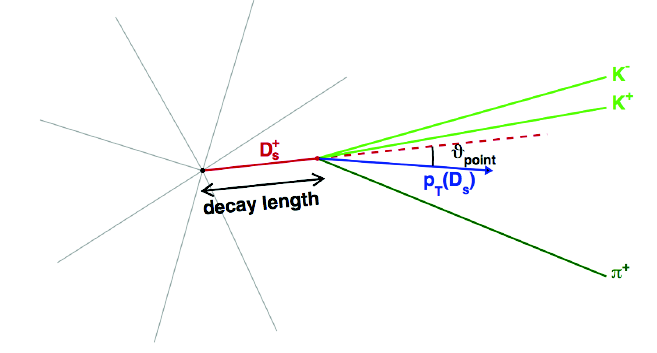
\includegraphics[width=12cm]{FigCap4/Ds.png}
\caption{Schematic view of the $\Dsplus\rightarrow \phi \pi^+ \rightarrow K^+K^-\pi^+$ decay.}
\label{fig:DsDecayTopology}
\end{figure}
To reconstruct and select $\Dsplus$ candidates, they have to pass
single-track quality cuts as well as selections of the decay topology
and of particle identification. In the following, details of each selection step will
be illustrated. 



\section{Single track selections}
Reconstructed tracks were selected by requiring:
\begin{itemize}
\item pseudo-rapidity $|\eta| < 0.8$
\item minimum $\pt > 0.3~\GeV/c$
\item at least 70 (out of a maximum of 159) associated space points in the TPC
\item $\chi^2/\mathrm{ndf} < 2$ in the TPC (where ndf is the number of degrees of 
freedom involved in the tracking procedure)
\item at least two (out of six) hits in the ITS, out of which at least one 
in either of the two SPD layers
\item ratio of crossed rows over findable clusters in the TPC larger than 0.8
\end{itemize}
The cuts at 70 TPC clusters and on the ratio of crossed rows over findable clusters in the 
TPC were applied to cure a difference between data and simulation 
in the track-selection criteria applied at the level of the AOD creation.
The distribution of these variables after applying the cuts 
are shown in Fig.~\ref{fig:singtrafter}, for the $\Dzero$-meson decay tracks.
\begin{figure}[!htbp]
\begin{center}
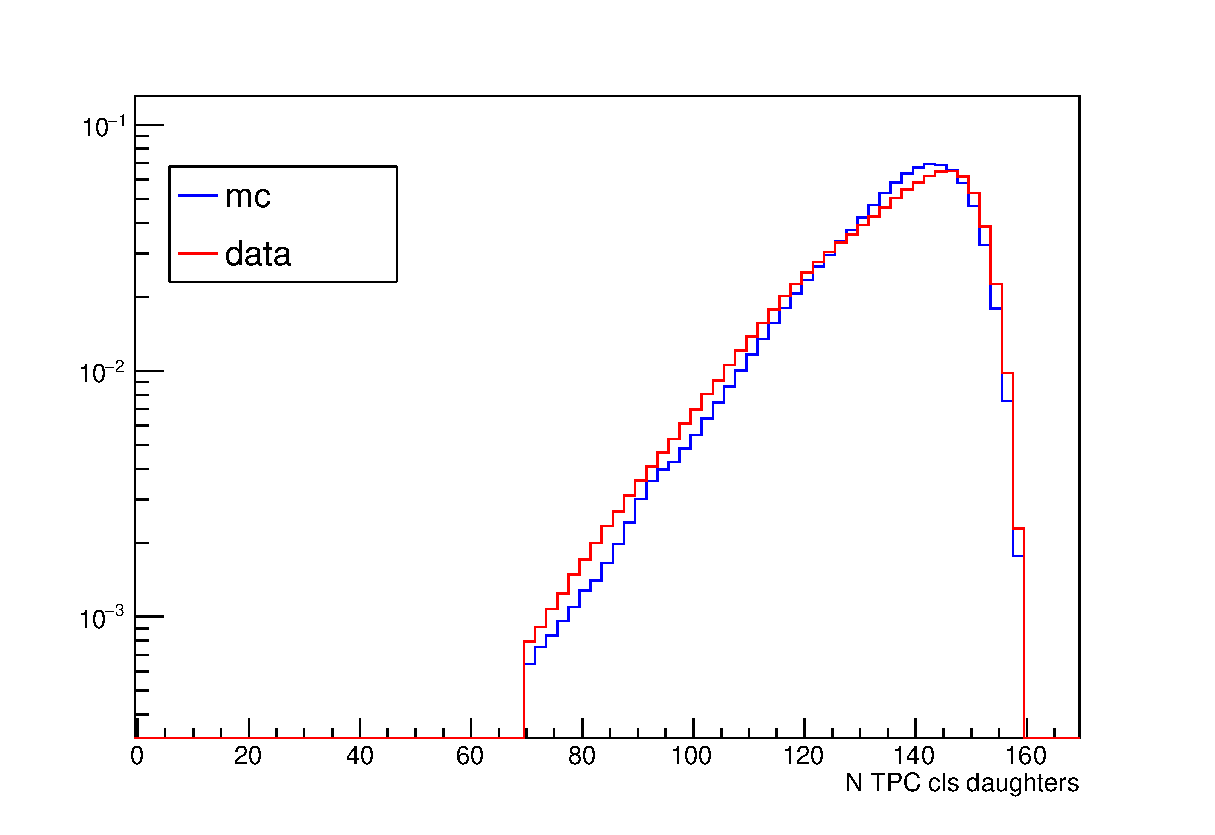
\includegraphics[width=.32\textwidth]{FigCap4/TPCclusters_AfterCut.eps}
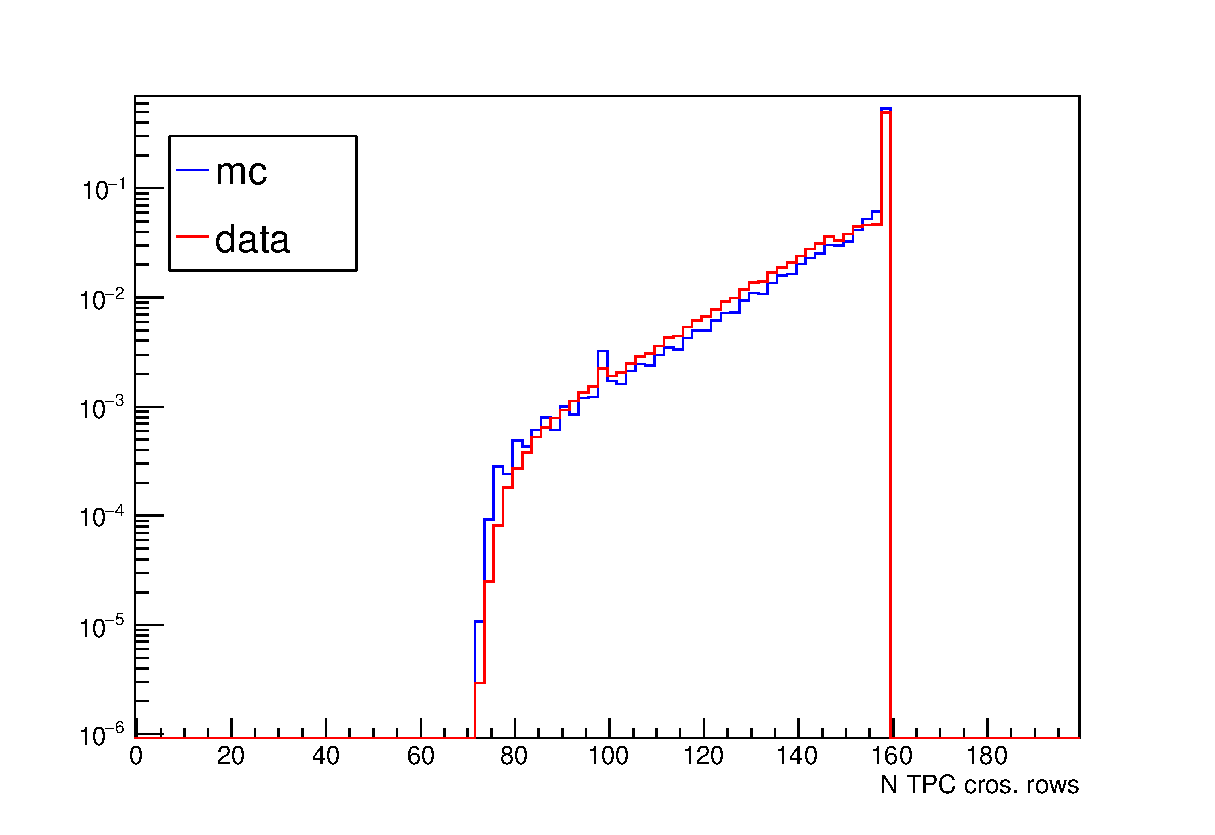
\includegraphics[width=.32\textwidth]{FigCap4/TPCcrossRows_AfterCut.eps}
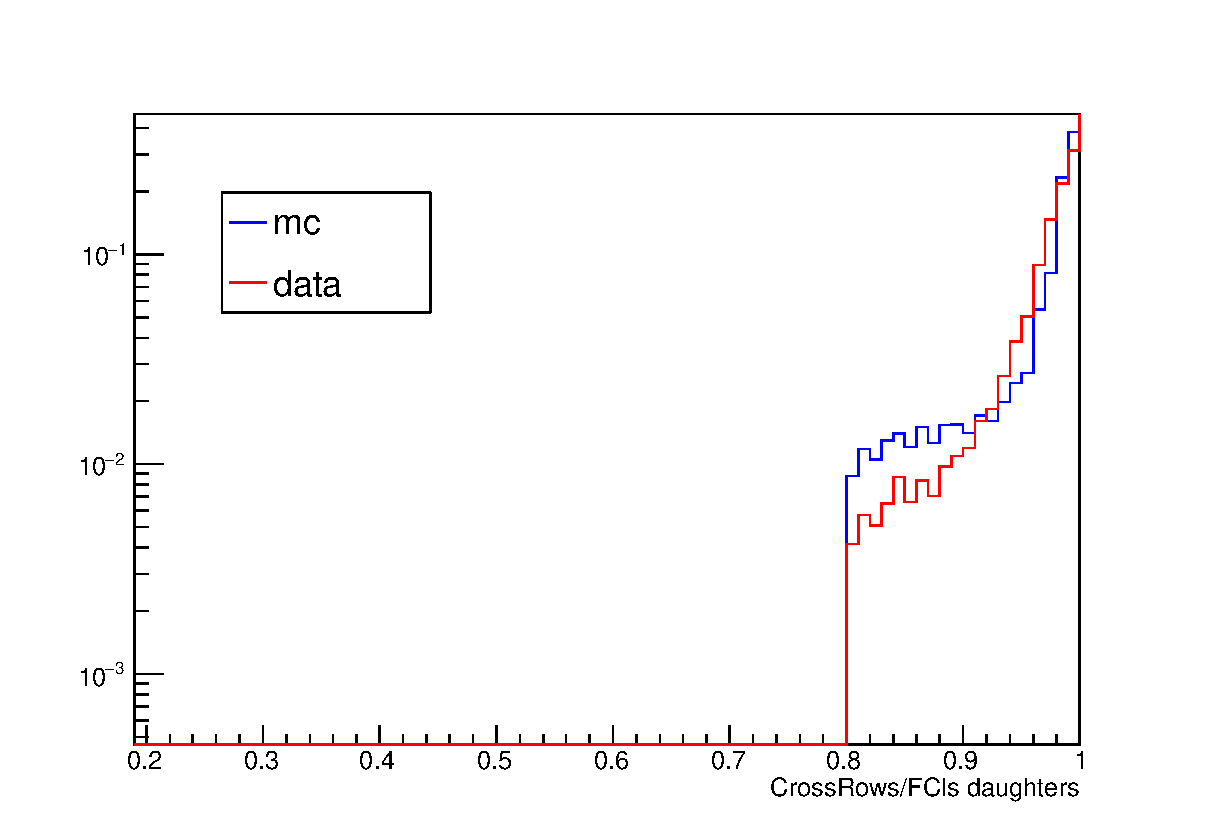
\includegraphics[width=.32\textwidth]{FigCap4/TPCCrossRowsFcls_AfterCut08}
\label{fig:singtrafter}
\caption{Distributions of number of TPC clusters (left), number of TPC crossed rows (middle) and
ratio of crossed rows over findable clusters (right) for $\Dzero$-meson daughter tracks 
passing the single-track selections described in the 
text, for data (red) and MC (blue).}
\end{center}
\end{figure}
For tracks that satisfy the above selection criteria, the transverse momentum 
resolution is better than 1$\%$ at $\pt = 1\, \Gevc$ and about 2\% at $\pt = 10 \, \Gevc$. 
The resolution on the track impact parameter, which is the distance of closest 
approach of the track to the primary vertex, is better than 75 $\mu$m for 
$p_t >$ 1 GeV/c for the projection on the bending plane ($r\phi$, normal to 
the beam direction) in pp collisions.
In order to have unbiased determination of the primary vertex, for each 
$\Dsplus$ candidate the interaction point was recalculated from the reconstructed 
tracks after excluding the candidate decay tracks.
\begin{figure}[!htbp]
\begin{center}
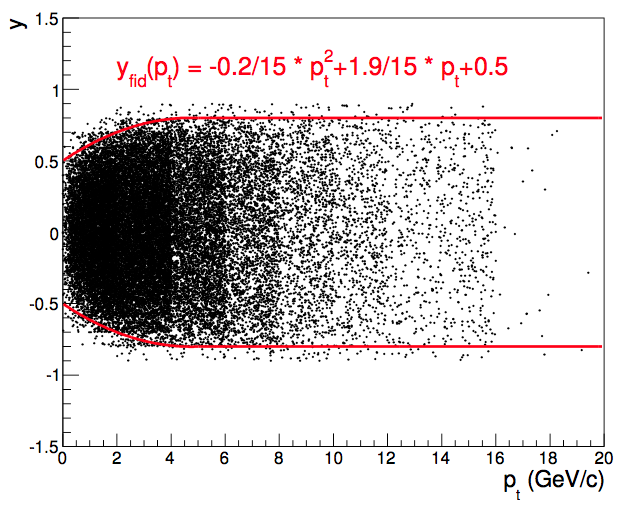
\includegraphics[width=.5\textwidth]{FigCap4/YvsPt.png}
\label{fig:singtrafter}
\caption{Rapidity versus $\pt$ distribution of the reconstructed $\Dsplus$ mesons. The fiducial acceptance region is defined by $|y| < y_{fid}(\pt)$.}
\end{center}
\end{figure}

The single-track selection criteria reduce the $\Ds$-meson acceptance, which drops 
steeply to zero for $|y| > 0.5$ at low $\pt$ and for $|y| > 0.8$ 
at $\pt > 5~\Gevc$. A $\pt$-dependent fiducial acceptance region was therefore defined as 
$|y| < y_{\mathrm{fid}}(\pt)$, with $y_{\mathrm{fid}}(\pt)$ increasing 
from 0.5 to 0.8 in the transverse momentum range $0 < \pt < 5~\Gevc$ 
according to a second-order polynomial function, and $y_{\mathrm{fid}}=0.8$ 
for $\pt > 5~\Gevc$.

\section{Decay-chain and topology selection}

The single-track selection provided a certain number of candidate
 decay tracks. Then, $D^{\pm}_s$ candidates were build from combinatorial 
 association of three candidate tracks, with the correct combination of charge 
 sign. In this way, a huge number of candidates was created, most of them 
 being combinatorial background. The goal is to separate background from
  $D^{\pm}_s$ signals (i.e. corresponding to real  $D^{\pm}_s$ decays). Candidates 
  are thus selected by applying topological cuts, specific to the meson and its 
  decay channel and varying as a function of the D meson $\pt$.
The main feature of the $\Dsplus$-decay topology is the presence of three tracks displaced from 
the primary vertex and compatible with the hypothesis of being originated from 
a common point. 
The variable that allows one to evaluate the displacement of a track is the 
impact parameter. The two most important detectors for the measurement
 of the impact parameter are the two SPD inner layers of the Inner Tracking System. \\
Below, the topological cuts used for $D^{\pm}_s$ signal selection
 are explained in detail. Plots in Fig.~\ref{fig:DL} of some of the listed variables complement
 the description, with distributions for signal and background extracted 
 from Monte Carlo production (PYTHIA) 
  and data and each one normalised to its number of entries. 
  New topological variables were introduced with respect to the 
  previous analysis of the same sample. They are the projections of the cosine of 
 Pointing angle and of the (normalized) decay length in the $xy$ plane 
 and the normalized impact parameter (IP)
resolution.
\begin{itemize}
\item \textbf{Decay length $D_{len}$}, defined as the distance between
 primary and secondary vertex. $D^{\pm}_s$ decay vertexes are displaced by
  a few hundred $\mu$m from the interaction vertex. Since real ${\rm D^{\pm}_s}$ 
  decay vertices have, on average, larger values of decay length than the
   background, this allows one to discriminate signal from background. 
   Likely cut values are $D_{len} > 300-400\, \mu $m;
\item \textbf{Cos$\theta_{point}$}, where $\theta_{point}$ is the angle
 between the momentum of the reconstructed $D^{\pm}_s$ meson and the 
 $D^{\pm}_s$ flight line (line connecting primary and secondary vertex, see
  Fig.~\ref{fig:image1}). The pointing angle is expected to be small for signal 
  candidates, resulting in a distribution of cos$\theta_{point}$ peaking at 1 for 
  signal and being broader for background candidates. Hence, cuts like the 
  one shown in fig. \ref{fig:distrib} (cos$\theta_{point} >$ 0.93 or tighter) 
  were usually applied to reject background;
\begin{figure}[!t]
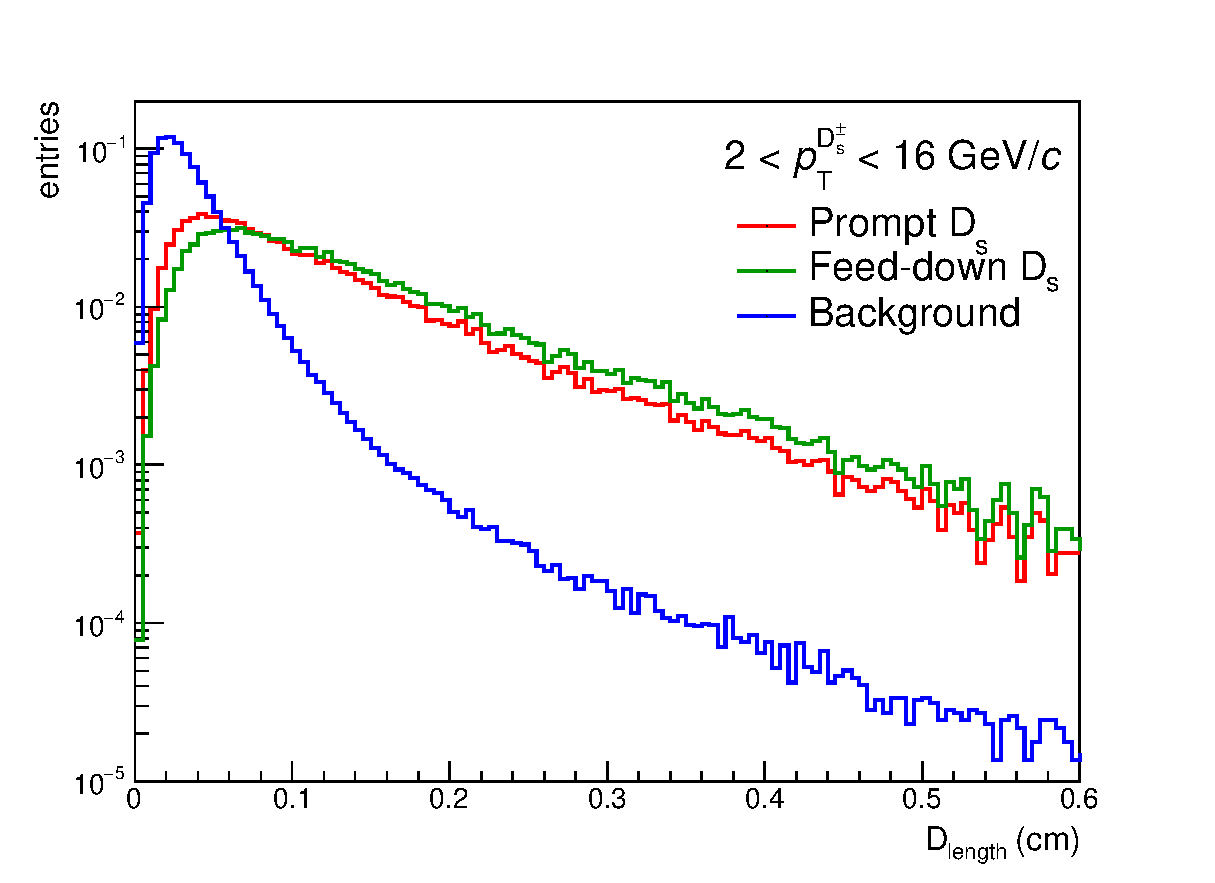
\includegraphics[width=6.5cm]{FigCap4/DL.eps}
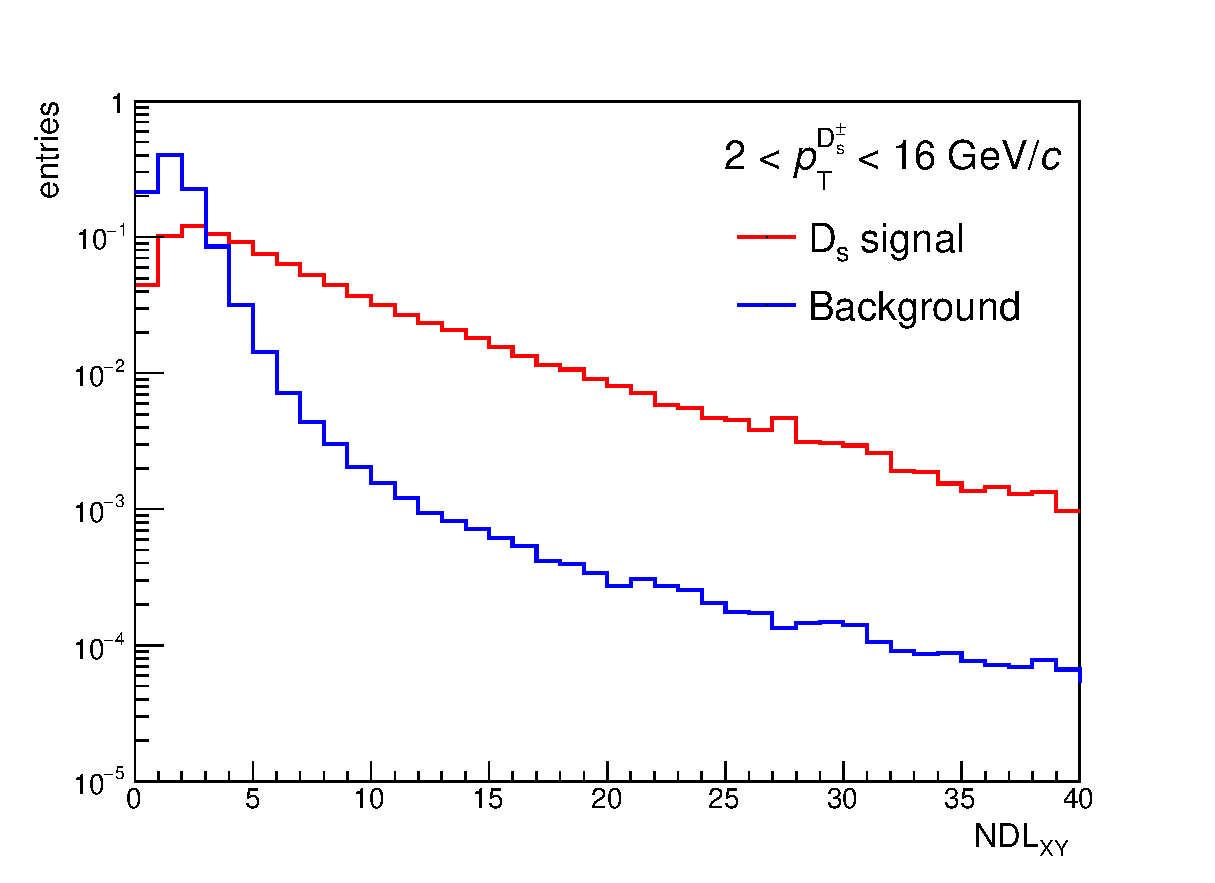
\includegraphics[width=6.5cm]{FigCap4/NDLxy.eps}
\caption{Distributions of decay length (left) and projection of decay length on the transerve plane (right) for signal (red) and background (blue) $D_s$ candidates in Pb-Pb collisions at $\sqrt{s}$=2.76 TeV in the range $4< p_t <12$ GeV/c obtained with a Monte Carlo simulation.}
\label{fig:DL}
\end{figure}

\begin{figure}[!t]
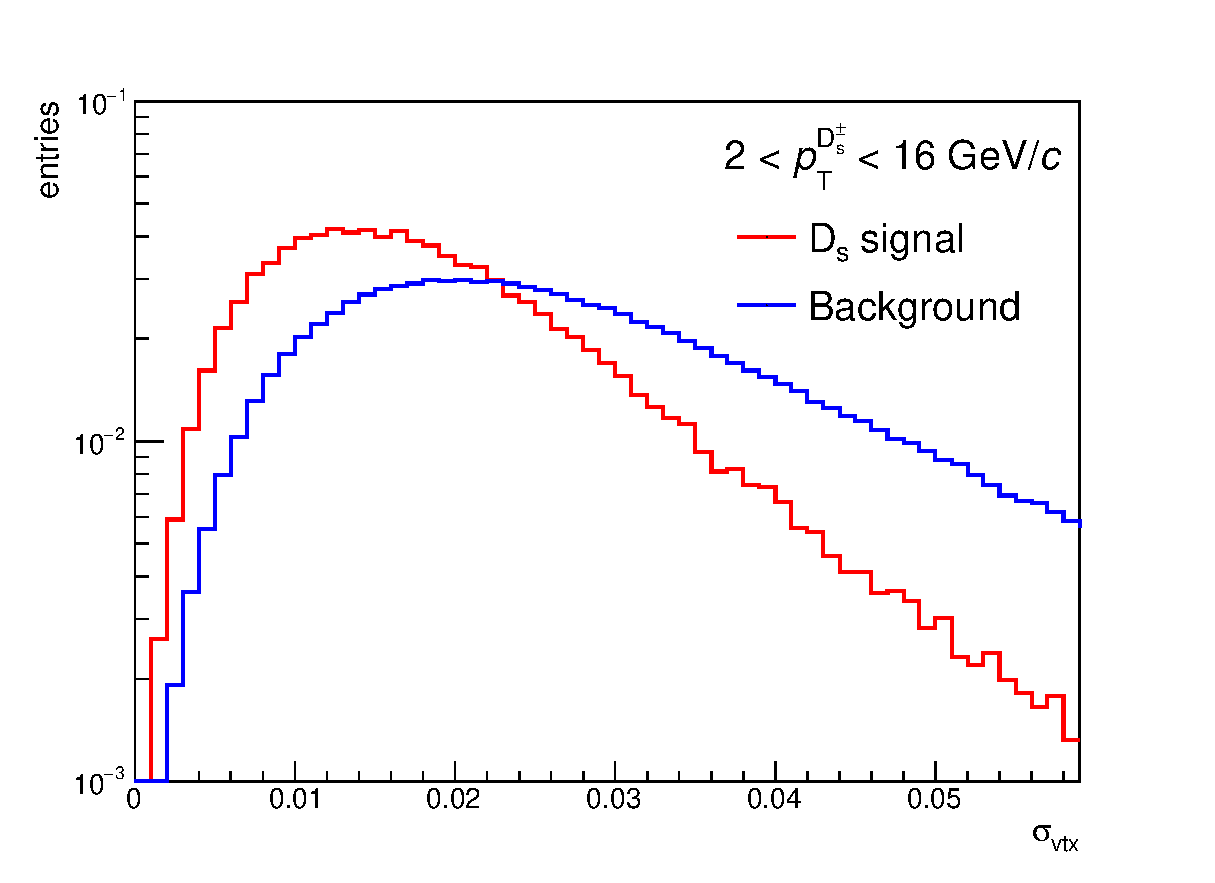
\includegraphics[width=6.5cm]{FigCap4/sigVert.eps}
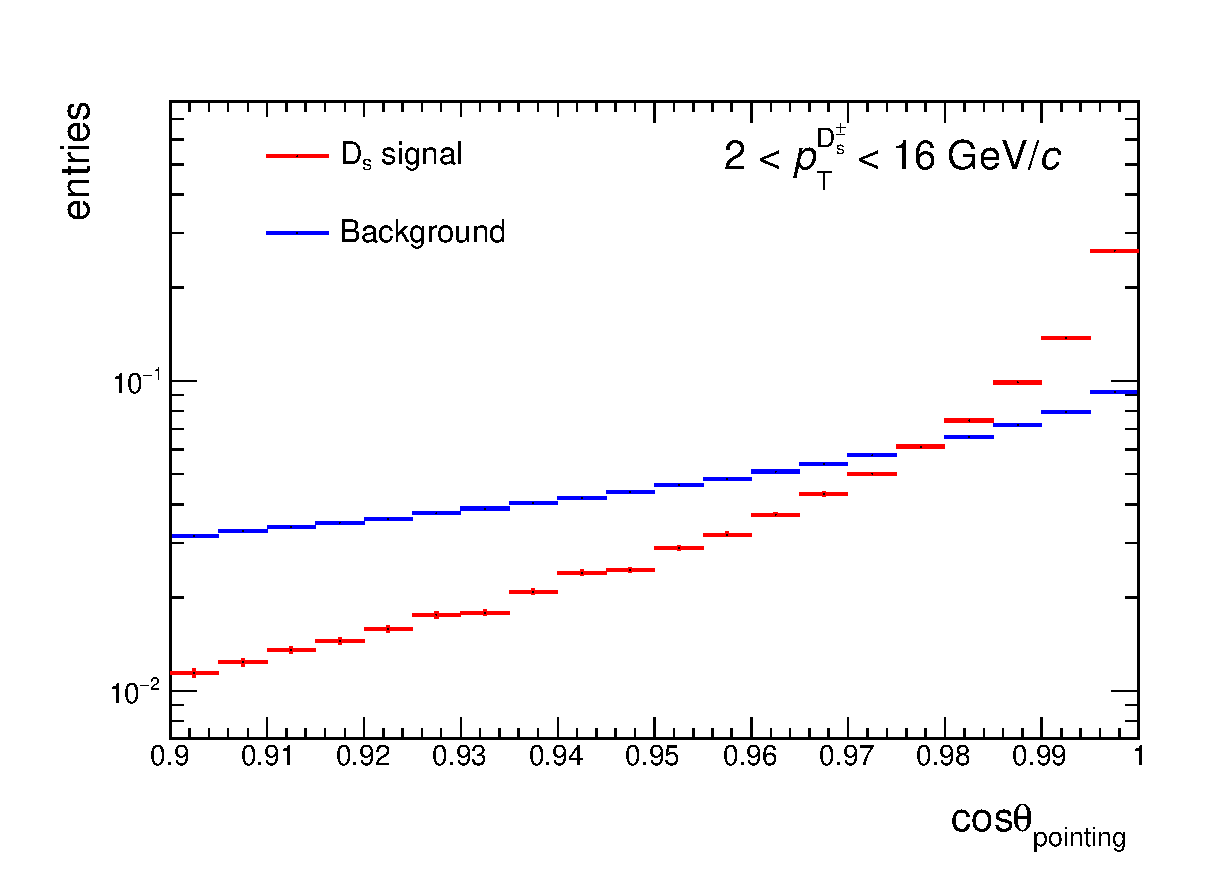
\includegraphics[width=6.5cm]{FigCap4/cosP.eps}
\caption{Distributions of decay length (left) and projection of decay length on the transerve plane (right) for signal (red) and background (blue) $D_s$ candidates in Pb-Pb collisions at $\sqrt{s}$=2.76 TeV in the range $4< p_t <12$ GeV/c obtained with a Monte Carlo simulation.}
\label{fig:DL}
\end{figure}

\item \textbf{track dispersion $\sigma_{vertex}$} around the decay vertex, defined as:
\[
\sigma_{vertex}=\sqrt{d^2_1+d^2_2+d^2_3}
\]
where $d_i$ is the distance of minimal approach between the decay 
track \textit{i} and the decay vertex. All tracks should originate from 
the secondary vertex, and $\sigma_{vertex}$ should be $\sim$ 0; in 
real cases, as a consequence of the tracking and vertexing resolution, 
the $\sigma_{vertex}$ has non-zero values and an upper cut is needed 
to exclude vertices made of random combination of tracks. Typical cut
 values on the track dispersion were between 0.02 $< \sigma_{vertex}<$ 0.05 cm;

\item \textbf{normalized decay length $L$}, defined as the decay length 
divided by its uncertainty;
\item \textbf{$\theta^*(\pi)$ angle}, it is the angle between the pion 
in the KK$\pi$ rest frame and the KK$\pi$ flight line. Cuts were applied
 on the distribution of the cos$\theta^*(\pi)$, with typical values 
 between 0.95 $<cos\theta^*(\pi)  <$ 1.0;
\item \textbf{$\theta'$(K) angle}, it is defined as the angle between
 one of the kaons and the pion in the KK rest frame. Cuts were 
 applied on the distribution of the $|cos^3(\theta'(K))|$, with typical 
 values between 0.0 $<|cos^3(\theta'(K))| <$ 0.05;
\item \textbf{Single track normalised impact parameter $IP$} : it is defined 
as the difference between the expected 
impact parameter value $d^{exp}_{0,r,\phi} \approx L_{xy} \cdot sin(\theta_{xy})$,
where $L_{xy}$ is the decay length on $xy$ plane and $\theta_{xy}$ is the angle 
between the reconstructed D meson and the charged particle on $xy$ plane, 
and the reconstructed one $d^{reco}_{0,r,\phi}$, then normalised by the square 
root of their respective uncertainties summed in quadrature. Since the 
distributions of the normalised IP resolutions are quite different for prompt 
and feed-down D mesons and background candidates, as can be seen in 
Fig.~\ref{fig:topomaticDplus} for the $\Dplus$ meson, a selection based on 
this variable can reduce the feed-down D-meson efficiency while keeping 
higher that of prompt D mesons. 
\end{itemize}

The selections on $\theta^*(\pi)$ and $\theta'$(K) angles have already 
been used in various experiments which measured $\Dsplus$ production 
like ZEUS \cite{Chekanov:2005mm} and ATLAS \cite{ATLAS:2011fea} as well as in previous ALICE
analysis of this sample and are based on kinematical 
considerations on the decay chain with a $\phi$ in the intermediate state.
Further selections were applied on the projections of the decay length, 
the normalized decay length and the cos$\theta_{point}$ in the transverse 
plane $xy$. The reconstruction of these parameters on the transverse plane 
allows indeed a better resolution than along $z$-axis.
The projections of the variables in the $xy$ plane are instead justified by 
the improving of the impact parameter resolution with respect to $z$-direction.\\


A further parameter which allowed to reduce the background is the
 \textbf{invariant mass of the reconstructed $K^+K^-$ pair}. This is not a topological 
 cut (i.e. a cut exploiting the displacement of the decay vertex), 
 but rather a selection on the decay chain. It is required that at least 
 one of the two pairs of tracks with opposite charge has an invariant
  mass compatible with the $\phi$ mass. The selection is done on 
  the absolute value of the difference between the $\phi$ 
   invariant mass from PDG and the reconstructed one:
\[
\Delta M = |M^{inv}_{rec}-M_{\phi}| 
\]
Typical values for cuts on the $\Delta M$ invariant mass 
are between 3 $<\Delta M<$ 15 MeV$/c^2$.

\begin{figure}[!t]
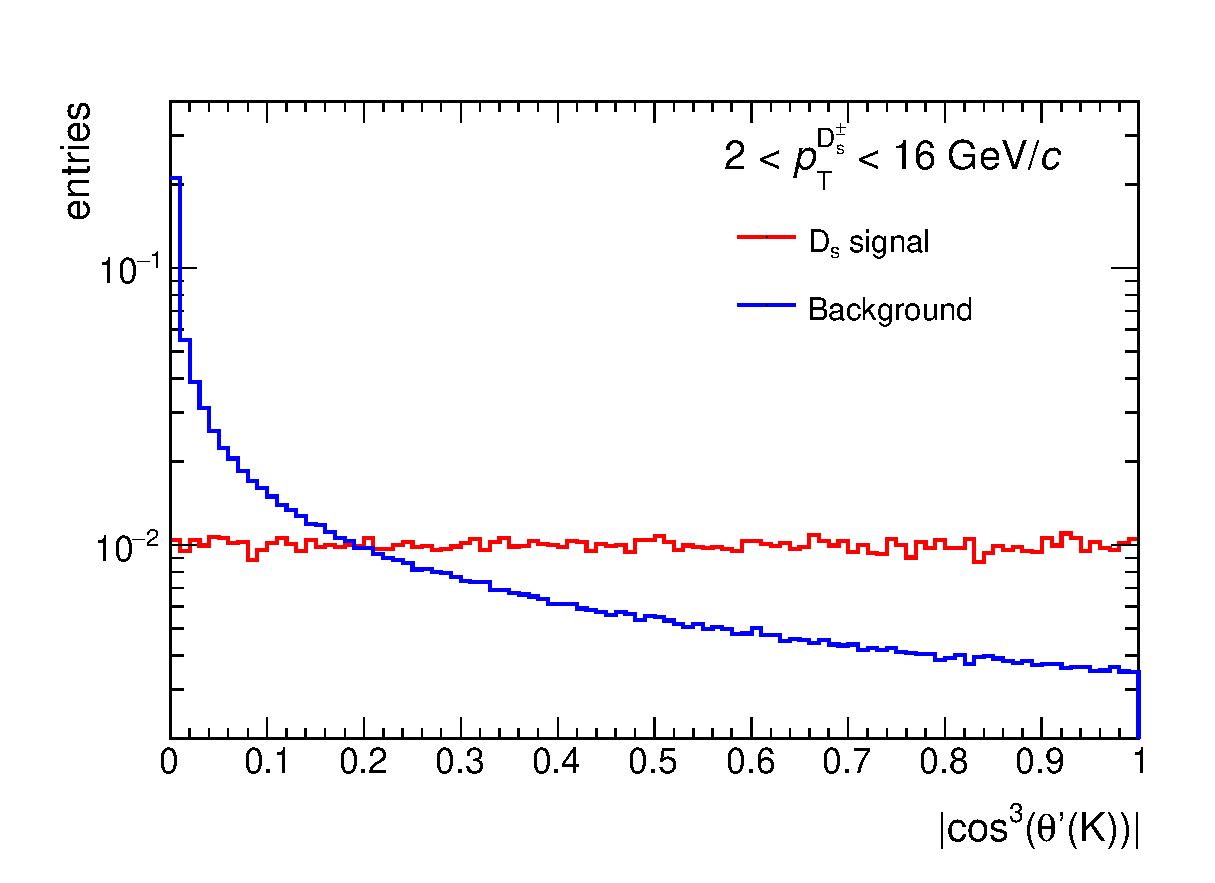
\includegraphics[width=6.5cm]{FigCap4/CosPiKPhi3.eps}
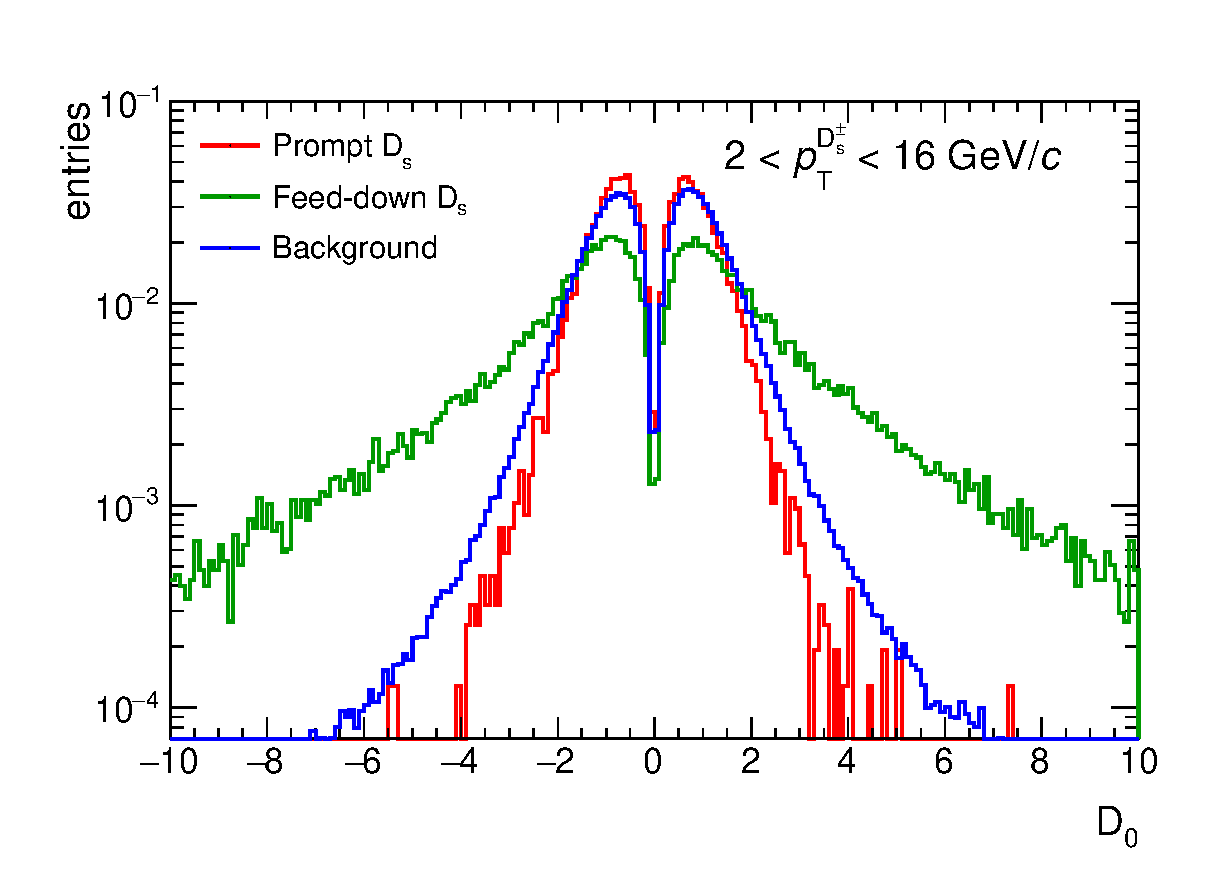
\includegraphics[width=6.5cm]{FigCap4/normIP.eps}
\caption{Distributions of cos$\theta_{point}$ (up, left), cos$\theta_{point,xy}$ (up,right) for signal and background $D_s$ candidates in Pb-Pb collisions at $\sqrt{s}$=2.76 TeV in the range $4< p_t <12$ GeV/c obtained with a Monte Carlo simulation.}
\label{fig:distrib}
\end{figure}

\section{Particle identification}
The Particle IDentification (PID) selection is based on the specific energy loss 
d$E$/d$x$ in the TPC and the time-of-flight from the interaction vertex to the 
TOF detector. This is used in the D-meson analysis to reduce the background, 
but it is essential for $\Dsplus$ studies because its signal-over-background
 ratios (S/B) of the order of a few percent.
A track is  considered compatible with a certain particle species 
(e, $\mu$, $\pi$, K or p) if the difference between the measured signal is
 within $n\sigma$ from the expected one for the various mass hypotheses
  with the theoretical predictions:
\[
|S_{meas}-S^{\pi,k,p}_{expected}| < n^{\pi,k,p}\sigma ,
\]
where $\sigma$ is the RMS of the Gaussian fit of the theoretical 
curve to the energy-loss or time-of-flight signals for each species.
Candidate triplets were required to have two tracks compatible with 
the kaon hypothesis and one with the pion hypothesis. In addition, 
since the decay particle with opposite charge sign has to be a kaon, 
a triplet was rejected if the opposite-sign track was not compatible 
with the kaon hypothesis. Usual values for PID cuts are between 
2-3 sigmas (more details in sec. 4.4.2).

\section{Invariant mass spectra and signal extraction}
For each candidate, two values of invariant mass can be computed, 
corresponding to the two possible assignments of the kaon and the 
pion mass to the two same-sign track. In fact, considering the $\Dsplus$
 decay, the charge configuration of the tracks (+, -, +) can be interpreted
  both as to ($K^+,K^-,\pi^+$) and ($\pi^+,K^-,K^+$). Signal candidates with 
  wrong mass assignement to the same-sign tracks would give rise to 
  a contribution to the invariant mass distributions that could introduce
   a bias in the raw yield of $\Dsplus$ mesons. It was verified, both in 
   data and in simulations, that this contribution is reduced to a negligible 
   level by particle identification selection and by the requirement that the
    invariant mass of the two tracks identified as kaons is compatible with 
    the $\phi$ PDG mass.

Once that the $\Dsplus$ candidates passed the selections they are 
used to fill invariant mass histograms of the in each $\pt$ interval.
This histogram is fitted by a function consisting of a sum of 
a Gaussian and an exponential function to describe the signal peak and 
the background shape respectively:
\begin{equation}
f(x)= Ae^{-B\cdot x}+Ce^{-\frac{(x-\mu)^2}{2\sigma^2}}.
\end{equation}
It is important to define the values of the cut parameters 
which allow to extract a stable signal. 
 The yield extraction was performed using a particle selection 
 strategy that has high efficiency and high statistical 
 significance for the D meson signal.
In order to choose the best set of topological cuts, 
the selected criterion is the maximisation of statistical 
significance defined as:
\[
Signif = \frac{S}{\sqrt{S+B}},
\]
where S and B are the extracted signal and background obtained 
from the fit procedure integrated within 3$\sigma$ 
around the peak of the Gaussian shape ($\sigma$ being the
RMS of the peak from the fit). The statistical significance is related to the 
relative statistical uncertainty on the extracted signal, so higher 
significance means lower statistical uncertainty on the raw yield. 
A second variable which is used in the cut optimisation procedure
 is the signal-over-background ratio S/B, as 
 an estimator of the powerfulness of the selection strategy. 
 The maximisation of the significance was required together
  with the request that the position of the peak and the width 
  of the Gaussian shape were compatible with the values
   obtained in simulated events, with the same selection strategy.
The topological variables have a certain degree of correlation among them. 
For this reason, for each $\pt$ interval, different parameters 
were simultaneously varied in wide ranges to consider all possible combinations. 
The selection values depend on the $\pt$ of the D-meson candidate and 
are detailed in Table~\ref{tab:cutsDs}.
\begin{table}[tbh!]
\centering
\begin{tabular}{|l|c|c|c|c|} 
\hline 
 $\Ds$ meson& \multicolumn{4}{c|}{pt interval (GeV/$c$)}\\
\hline
 & 2--4  & 4--6 & 6--8 & 8--12\\
\hline
Decay length ($\mum$)        & $>$300 & $>$350 & $>$350 & $>$400\\
Decay length XY ($\mum$)     & $>$0 & $>$200 & $>$200 & $>$200\\
Norm Decay length XY          & $>$2.0& $>$0.0 & $>$2.0 & $>$2.0\\
Cosine pointing              & $>$0.94 & $>$0.95 & $>$0.95 & $>$0.97\\
$\sigma_{vertex}$  (cm)          & $<$0.02 & $<$0.03 & $<$0.03 & $<$0.06\\
M$^{\phi}_{inv}$ - M$^{\phi PDG}_{inv}$ (MeV/$c^{2}$) & $<$8.0 & $<$10.0 & $<$4.5 & $<$9.0\\
$\cos \theta^*(\pi)$    & $<$1.0 & $<$1.0 & $<$1.0 & $<$0.95\\
$|\cos^3 \theta^\prime({\rm K})|$        & $>$0.10 & $>$0.05 & $>$0.05 & $>$0.05\\
Norm. IP residual Kaon  & $<$2.5 & $<$2.0 & $<$2.0 & $<$2.0 \\
Norm. IP residual Pion  & $<$2.5 & $<$2.0 & $<$2.0 & $<$2.0 \\[1ex]
\hline
\end{tabular}
\caption{Selections used for the $\Ds$ meson in the four transverse momentum intervals considered.} 
\label{tab:cutsDs}
\end{table}
In Fig.~\ref{fig:invmassDs} the invariant mass distributions 
in four $\pt$ bins for $\Ds$ mesons are shown.
\begin{figure}[!htb]
\begin{center}
 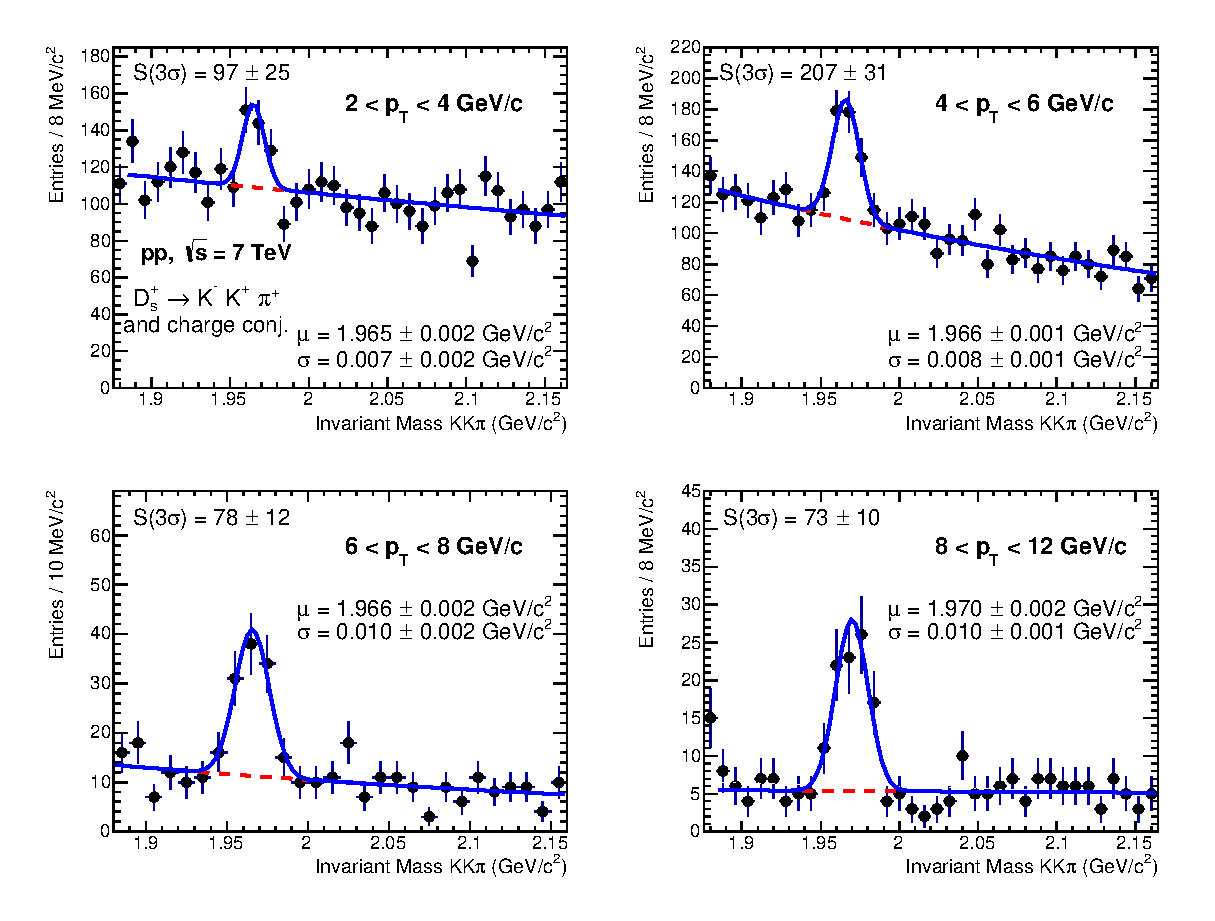
\includegraphics[width=.99\textwidth]{FigCap4/DsMassHistos_ppPass4.eps}
\caption{Invariant mass distributions of $\Ds$ candidates and charge
conjugates in the four considered $\pt$ intervals.}             
\label{fig:invmassDs}
\end{center}
\end{figure}
An indication of the improved resolution provided by the new 
reconstruction of the sample is shown in Fig.~\ref{fig:sigma4vs2}, where the 
Gaussian sigma of the invariant mass fit is shown in comparison with 
results of the previous reconstruction, for both data and MC. 
\begin{figure}[!hb]
\begin{center}
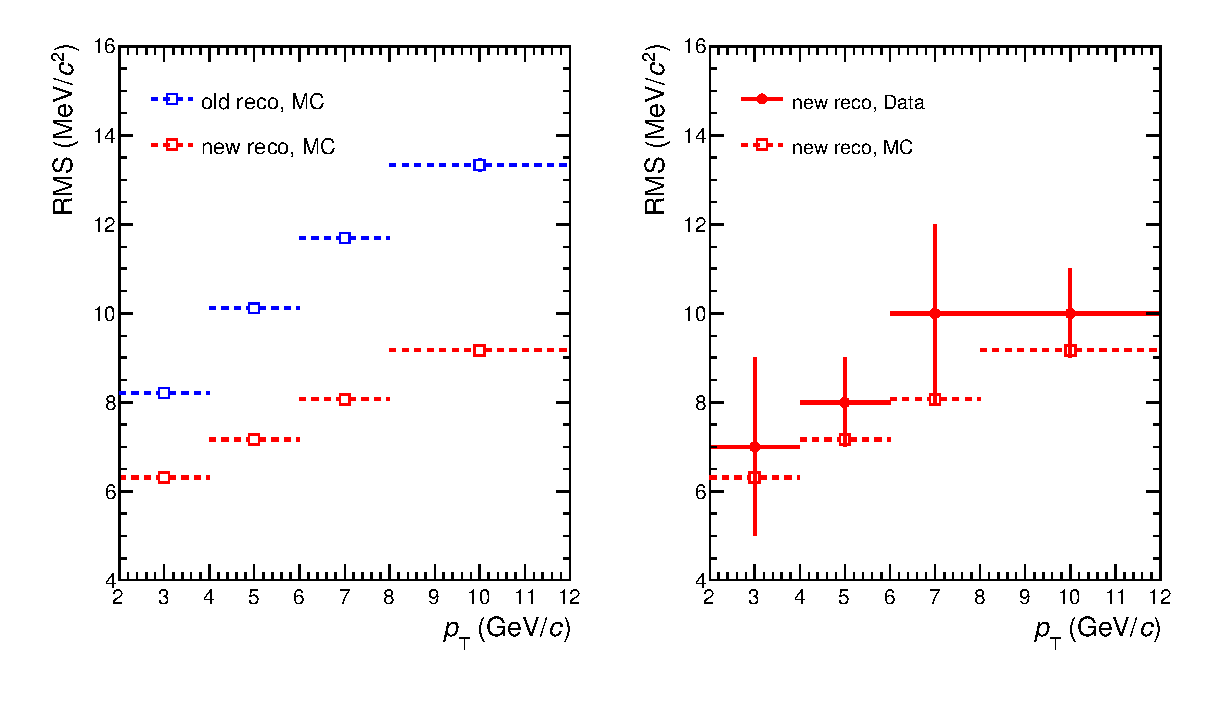
\includegraphics[width=.48\textwidth]{FigCap4/Resolutions_pass2_pass4.eps}
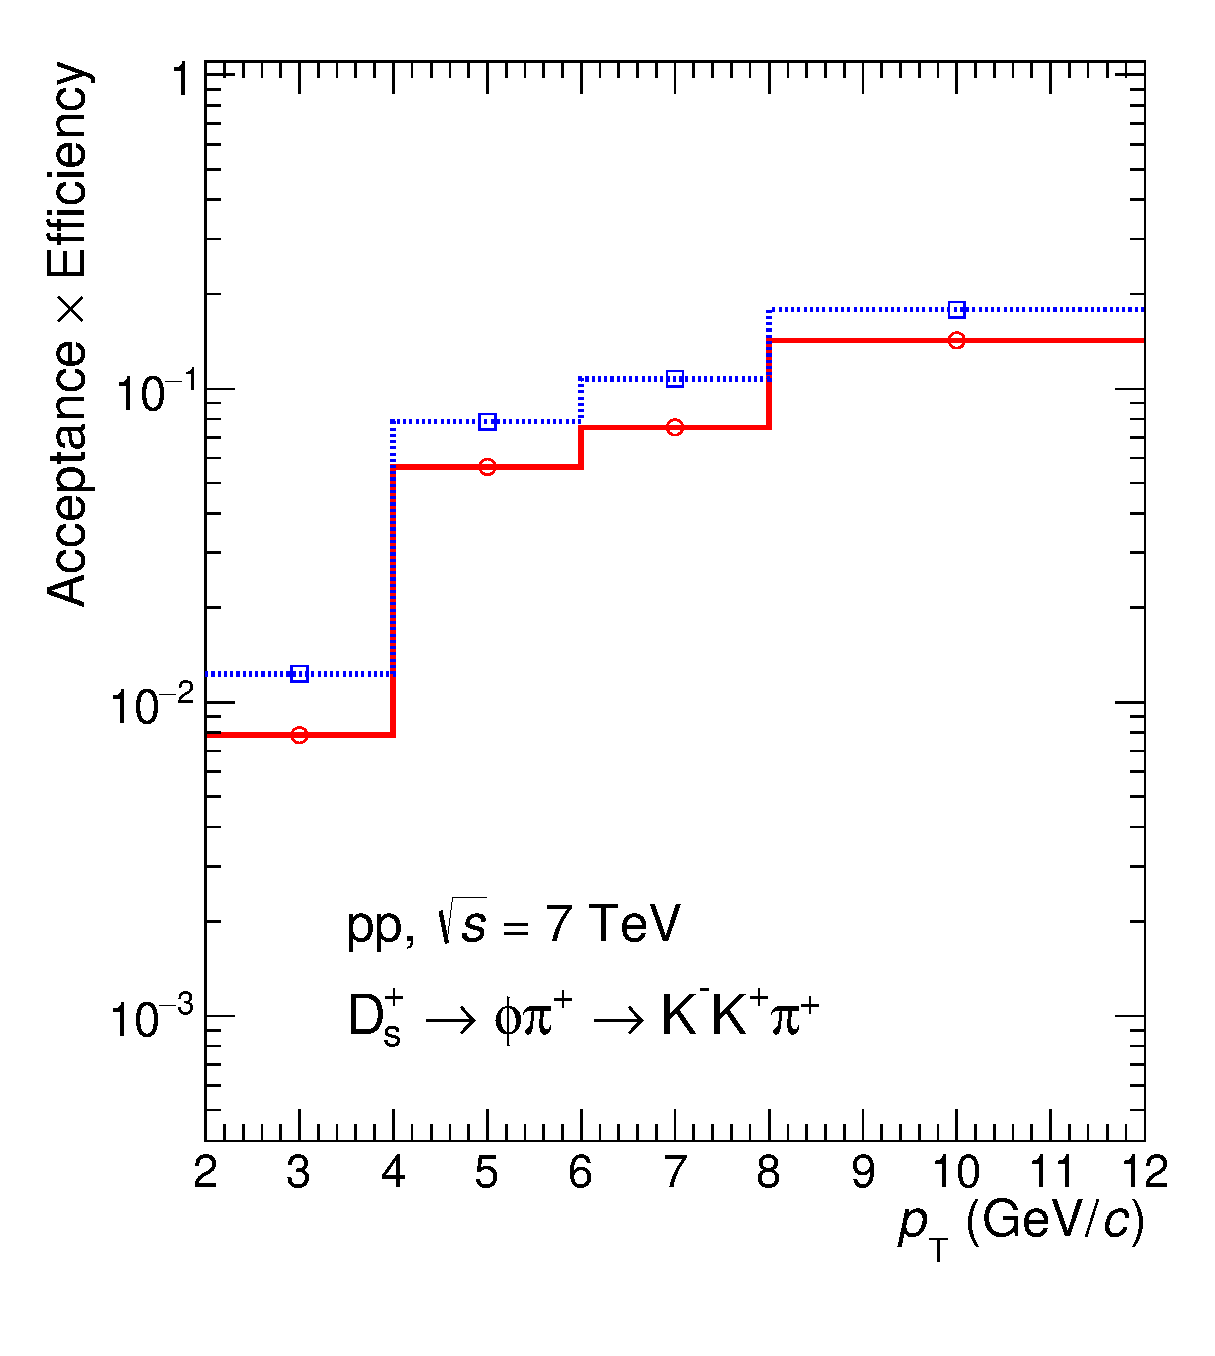
\includegraphics[width=.48\textwidth]{FigCap4/AccEff_Ds_Pass4.eps}
\caption{Left: Gaussian width of $\Dplus$, $\Ds$ peak in pass4 and pass2 reconstructions and
corresponding simulated samples. Right: Acceptance-times-efficiency of prompt and feeddown $\Ds$ mesons.}
\label{fig:sigma4vs2}
\end{center}
\end{figure}

\section{Corrections}

The $\Ds$ raw yields extracted from the fits to the invariant-mass distributions
were corrected to obtain the $\pt$-differential production cross sections of prompt 
(i.e.\ not coming from weak decays of B mesons) D mesons.
The production cross section
was calculated as:
\begin{equation}
  \label{eq:dsdpt}
  \left.\frac{{\rm d} \sigma^{\rm D^{+}_{\rm s}}}{{\rm d}\pt}\right|_{|y|<0.5}=
  \frac{1}{ \Delta \pt}\frac{1}{{\rm BR} \cdot L_{\rm int}}\frac{\left.f_{\rm prompt}(\pt)\cdot \frac{1}{2} N^{\rm D^\pm_{\rm s}~raw}(\pt)\right|_{|y|<y_{\rm fid}}}{ 2 y_{\rm fid}(\pt) \,({\rm Acc}\times\epsilon)_{\rm prompt}(\pt)}\,,
\end{equation}
where $N^{\rm D^\pm_{\rm s}~raw}(\pt)$ is the value of the raw yield 
(sum of particles and antiparticles),
 which need to be corrected for the B-meson decay feed-down contribution 
(i.e.\ multiplied by the prompt fraction $f_{\rm{prompt}}$), divided by the 
acceptance-times-efficiency for prompt $\Ds$ mesons, 
$(\rm Acc \times \epsilon)_{\rm{prompt}}$, and divided by a factor of two to 
obtain the charge (particle and antiparticle) averaged yields.
The corrected yields were further divided by the decay channel branching ratio (BR), 
the $\pt$ interval width ($\Delta \pt$), the rapidity coverage 
($2 y_{\rm fid}$) and the integrated luminosity $L_{\rm int}$.
The integrated luminosity as computed as $L_{\rm int} = N_{ev}/\sigma_{pp,MB}$,
where $N_{ev}$ is the number of analysed events and 
$\sigma_{pp,MB} = 62.2$ mb~\cite{Abelev:2012sea}
is the cross-section for the minimum-bias trigger condition, derived from
a Van-der-Meer scan measurement.

\subsection{Reconstruction and selection efficiency}
The acceptance and efficiency correction factors, 
$(\rm Acc \times \epsilon)$, were determined for the $\Ds$-meson
hadronic decay considered in this analysis using Monte Carlo simulations 
of pp collisions generated with the PYTHIA 6.4.21 event generator~\cite{Sjostrand:2006za} with the 
Perugia-0 tune\cite{Skands:2010ak}, and particle transport through the apparatus 
using GEANT3~\cite{Brun:1994aa}.
The luminous region distribution and the conditions (active channels, gain, 
noise level and alignment) of all the ALICE detectors were included in the 
simulations, considering also their evolution over time during the 2010 LHC 
data taking period.
In the production, only events containing a $c\bar{c}$ or a $b\bar{b}$ pair 
were transported through the apparatus and reconstructed and
D mesons were forced to decay hadronically via the decay channel relevant to
the specific analysis.
The efficiency was extracted separately for prompt D mesons and D mesons 
from $b$-hadron decays.
The $(\rm Acc \times \epsilon)$ of $\Ds$-meson reconstruction and
selection is shown in Fig.~\ref{fig:effDs}. In the left panel, the efficiency 
for prompt D mesons is shown before and after PID 
selection. One can see that the particle identification allows to keep 
around 90\% of the signal. D mesons from beauty decay 
have higher efficiency than
the prompt ones in all the $\pt$ intervals, due to the more displaced 
decay vertex from interaction point.
In general, with the chosen topological selections, efficiencies in this analysis
are on average 15\% lower than those used in the previous reconstruction. 
The present analysis uses more powerful selection variables 
(projections on $xy$ plane and impact parameter residual) that
enhance the signal-over-background ratio for $\Ds$ meson by a factor 
from 2 to 5 depending on the $\pt$ interval, with an acceptable worsening
of the global efficiency. Large signal-over-background ratios are essential 
to assure a good stability of the extracted yield.

\subsection{B-feeddown subtraction}

The $f_{\rm prompt}$ fraction was calculated using the B production cross sections from  
FONLL calculations~\cite{Cacciari:1998it, Cacciari:2001td}, the 
$\mathrm{B} \rightarrow \mathrm{D} + X$ decay kinematics from the EvtGen package~\cite{Lange:2001uf} 
and the efficiencies for feed-down D mesons reported in 
Fig.~\ref{fig:AccEff}:
\begin{equation}
\label{eq:fpr}
f_{\mathrm{prompt}} =1- \frac{N^{\text{D~feed-down}}_{\mathrm{raw}}}{N^{\mathrm{D}}_{\mathrm{raw}}}= 1- \left (\frac{\rm d^2 \sigma}{\mathrm d\pt \mathrm d y} \right)^{\rm FONLL}_{\text{feed-down}} \cdot \frac{(\mathrm{Acc} \times \epsilon)_\text{feed-down} \cdot \Delta y \Delta \pt \cdot \mathrm{BR} \cdot L_{\rm int}}{N^{\rm D +\overline{D},raw}/2}\,,
\end{equation}
where the $\pt$ dependence of $f_{\rm prompt}$, $N^{\rm D +\overline{D},raw}$ and
$(\mathrm{Acc} \times \epsilon)_\text{feed-down}$ is omitted for brevity.
The values of $f_{\rm prompt}$ range between 0.85 and 0.97 depending on 
D-meson species and $\pt$.



\section{Systematics}
In this section the study of the systematic uncertainties for the
 measurement of the $\Dsplus$ yield as a function of $\pt$. 
 The contributions to the systematic uncertainty from different 
 sources were studied separately and described in detail in the following.

\subsection{Raw yield extraction}
Systematics on the yield extraction were evaluated by studying 
the variation of the raw yields in each $\pt$ interval when 
varying the signal line shape
(Gaussian pole and sigma values) and the fitting function for the 
background. Let's examine these two contributions separately.

\emph{Signal line shape}
The uncertainty on the signal was calculated by considering the combinations among these fit
variations: (i) free width parameter, (ii) free mean parameter, (iii) varying width parameter
by 20\% with respect to MC value, (iv) fixing width parameter to MC value, (v) fixing mean parameter to MC value.
The error was extracted as the maximum error ((max. value - min. value)/2) divided by square root of 12.\\
It results in a 5\% systematic uncertainty in all the $\pt$ intervals.

\emph{Background fit function}
Using different functions to fit the background could in 
principle introduce some bias in the yield extraction. 
The default shape used to give the central yield is an 
exponential function, but linear and second 
order polynomial shapes were also tested. In Table~\ref{tab:chi2bkg} 
the values of reduced chi square referred to the compatibility 
of the background function with data (excluding peak region) are 
reported. One can see that all the three shapes 
give a good description of data, but in general no improvements 
are visible when adding more parameters in the fit
with respect to exponential shape, so the latter confirms itself as a good choice.
Neverthless, it is important to look also at the values of the 
extracted yield to assess about possible biases.
 In order to do this, 50 simulated samples (generated via 
 Poissonian smearing from
the exponential background taken from data) were fitted
 with different background functions. Yields extracted with exponential 
 background were compared with those using linear and 
 polynomial functions with the same
configuration for pole, sigma, mass range and bin width. 
A potential shift from zero of the mean of the resultant distribution 
 should reveal the bias from the change of background. The
  spread of the distribution, instead, is only due to statistical fluctuations,
 as it originates from variations in mass range and bin width. In the 
 top panels of Fig.~\ref{fig:diffBkgPt0},~\ref{fig:diffBkgPt1},~\ref{fig:diffBkgPt2},~\ref{fig:diffBkgPt3} 
 the relative difference of the yields 
 extracted with linear or Pol2 shapes with that using an e
 xponential can be seen for the 4 $\pt$ intervals.
 The shift in the distribution is not statistically significant 
 ($< 3\sigma$ ) in all the $\pt$ intervals. 
 In the bottom panels of the same figures, it is plotted the 
 difference of the mean yields with different
backgrounds for each of the 50 samples, in number of significative 
sigmas of the yield distribution for exponential background.
 Again, one can see that the significance is always less than 1, 
 confirming that different
background fit functions do not introduce systematic 
effects on yield extraction.\\
 \\
The systematic from the yield extraction is hence a 5\%. 
It results reduced by a factor 3-4 with respect to the analysis of pass2,
where it was around 15-20\% depending on the $\pt$ interval. 

\begin{table}[!t]
\centering
\vspace{0.5cm}
\begin{tabular}{|c|c|c|c|c|} 
\hline \rule{0pt}{2.7ex}
 & $\pt$ interval & Exponential & Linear & Pol2 \\ 
 &(GeV/$c$) & & &  \\ 
\hline \rule{0pt}{2.7ex}
           &\phantom{0}2--4\phantom{0} & 1.21 & 1.21 & 1.09\\
           $\chi^2$ &\phantom{0}4--6\phantom{0} & 1.15 & 1.18 & 1.16\\
          &\phantom{0}6--8\phantom{0} & 1.03 & 1.02 & 1.03\\
           &\phantom{0}8--12 & 0.99 & 0.99  & 1.03\\
\hline

\end{tabular}
\caption{$\chi^2$ values for the fit of the background (peak region excluded) in the
considered $\pt$ intervals of the $\Ds$ meson.} 
\label{tab:chi2bkg}
\end{table}

\begin{figure}[!htb]
\begin{center}
 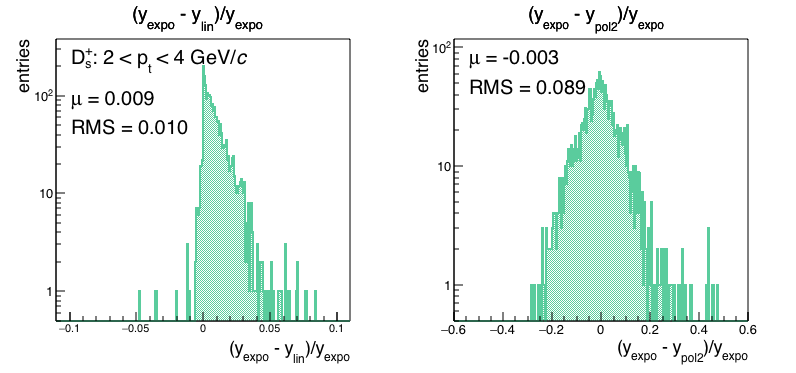
\includegraphics[width=.70\textwidth]{FigCap4/studyBkg_Free_pt0.png}
\caption{Relative difference of signal yield with exponential and linear (left) and Pol2 (right) 
functions for background for $2 < \pt < 4 ~\Gevc$.}             
\label{fig:diffBkgPt0}
\end{center}
\end{figure}


\subsection{Selection efficiency}

The systematic uncertainty due to possible imperfections
 in the description in the simulations
of the variables used in the geometrical selections of the 
D-meson displaced decay vertices was
studied by repeating the analysis varying the applied selection criteria.
The systematics on selection efficiency want to account for 
possible imperfections in the MC description ($\pt$, 
impact parameter ... resolution distributions) which could 
cause a bias in the final yield when correcting for the efficiency terms.
Hence, different sets of cuts were exploited and corrected 
yields obtained with sets of cuts with medium-high significance 
values were compared. Twelve sets of cuts were compared, 
with their respective efficiencies spanning a variation of
a factor from 2 to 6, depending on the $\pt$ interval. For this 
reason, we are allowed to take the RMS of the corrected yield distribution as 
an estimator for the systematic uncertainty. \\New topological 
variables were introduced with the re-analysis of this
sample, like the projection on xy plane of the cosine of Pointing 
angle and of the decay length of the candidate, or like
the normalized decay length (decay length divided by its error) 
and its projection on xy plane and the normalized impact parameter
residual. \\In Fig.~\ref{fig:cutVariation} (left) one can see the 
distribution of the ratio of corrected yields with different selections with respect to the one
used to give the central value, in different colours for each 
$\pt$ interval. The RMS of each distribution is reported on the plot. 
We decided to give a smoothed value on $\pt$ for these uncertainties, 
setting them to 7\% everywhere.\\
We also looked at the possible contribution to this systematic from
 variations in the xy impact parameter distribution 
of the particles. By changing the MC distribution by up to a 10\% 
variation, the variation of the efficiencies
of the previously analysed 12 sets of cuts results in less than 3\%. 
So, such variation is included in the already quoted 7\% from topological
selection. In Fig.~\ref{fig:cutVariation} (right) there is an example of the 
effect on the decay length distribution with and without the smearing on
resolution, for signal and background. A small shift in the distribution 
is evident at low $\pt$. In Fig.~\ref{fig:DLwoSmear} there is instead the ratio
of efficiencies after and before the smearing, for the case of 10\% 
variation with respect to the original xy impact parameter resolution.\\
In this case, we reduce by a factor of 2 the uncertainty quoted for pass2 analysis.

\begin{figure}[!htb]
\begin{center}
 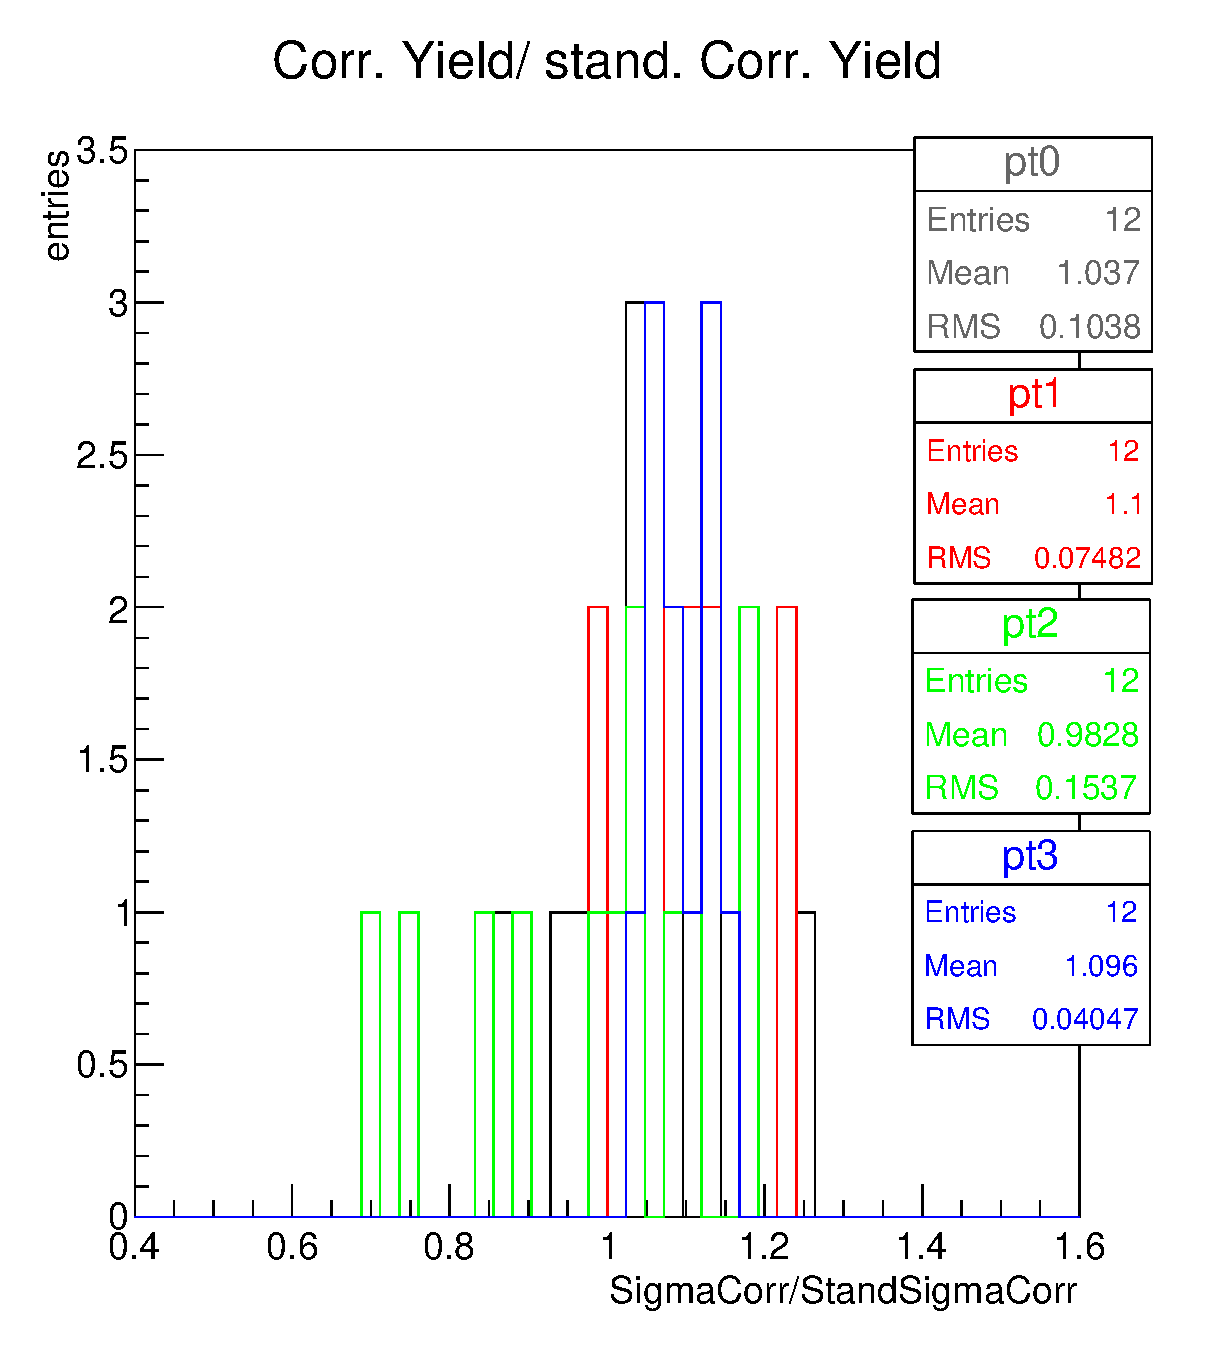
\includegraphics[width=.44\textwidth]{FigCap4/rms_cutvariation.eps}
 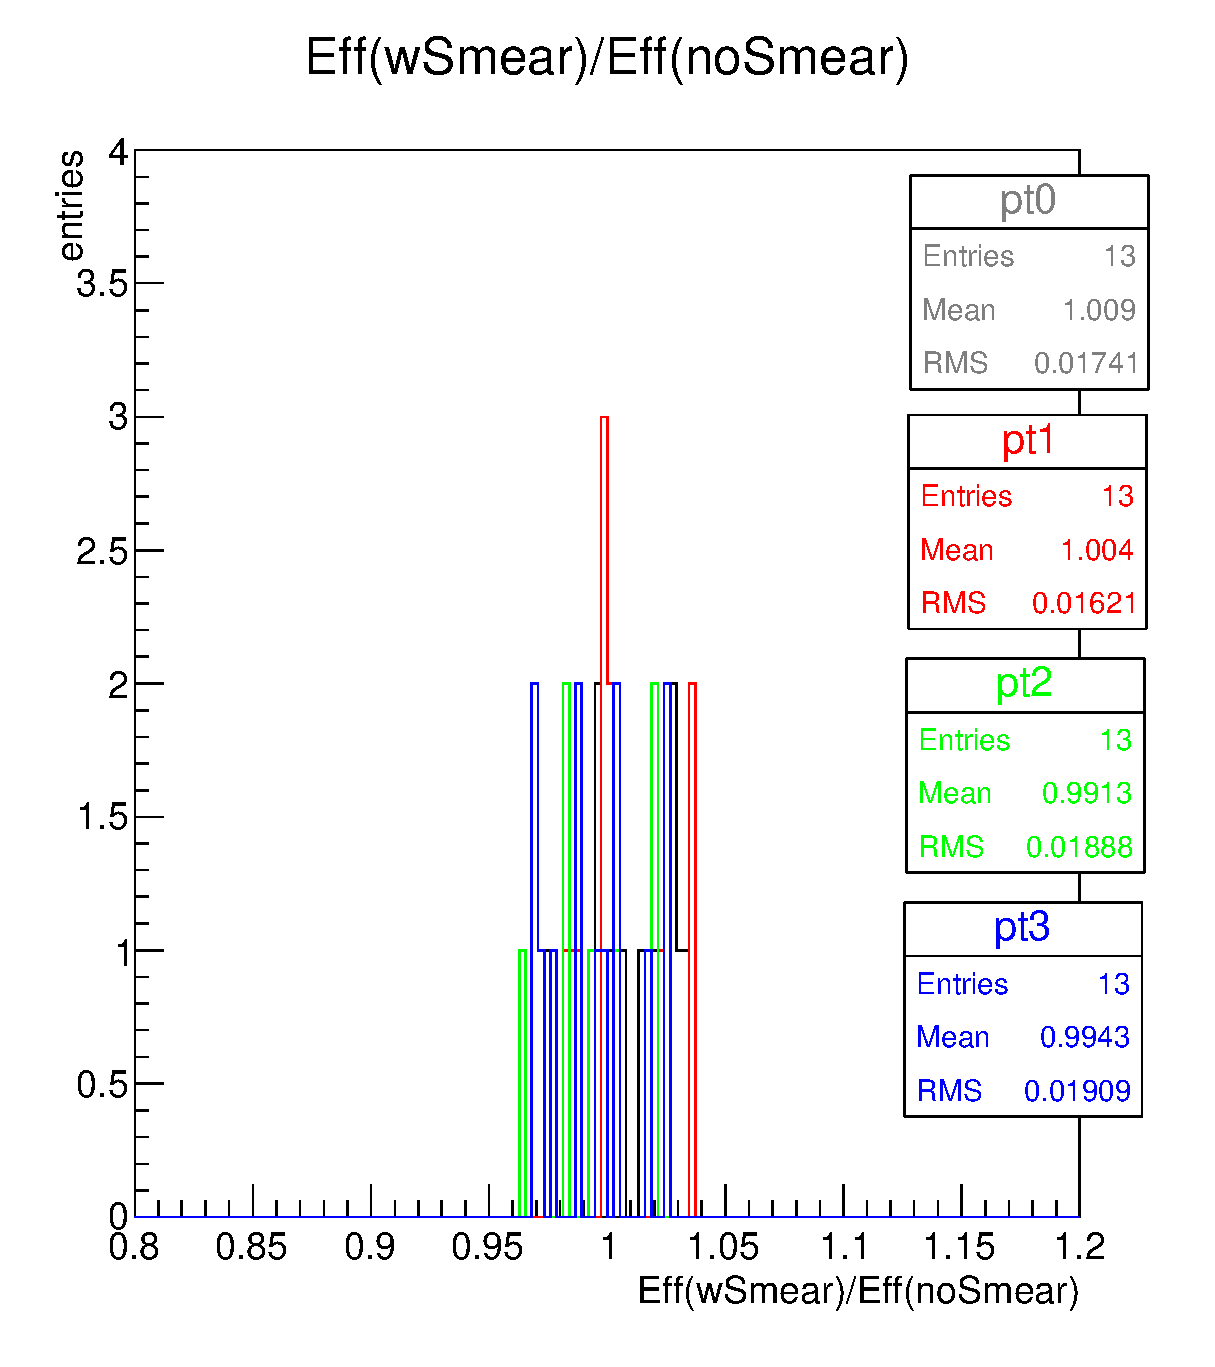
\includegraphics[width=.44\textwidth]{FigCap4/rms_smearp10.eps}
\caption{Left: $\Ds$ corrected yield measured with 12 different sets of
cuts and compared to the yield from the best set of cuts (chosen for the central yield value). Right: ratio for $\Ds$ efficiencies w/o a 
10\% smearing on the xy impact parameter resolution.}             
\label{fig:cutVariation}
\end{center}
\end{figure}

\begin{figure}[!htb]
\begin{center}
 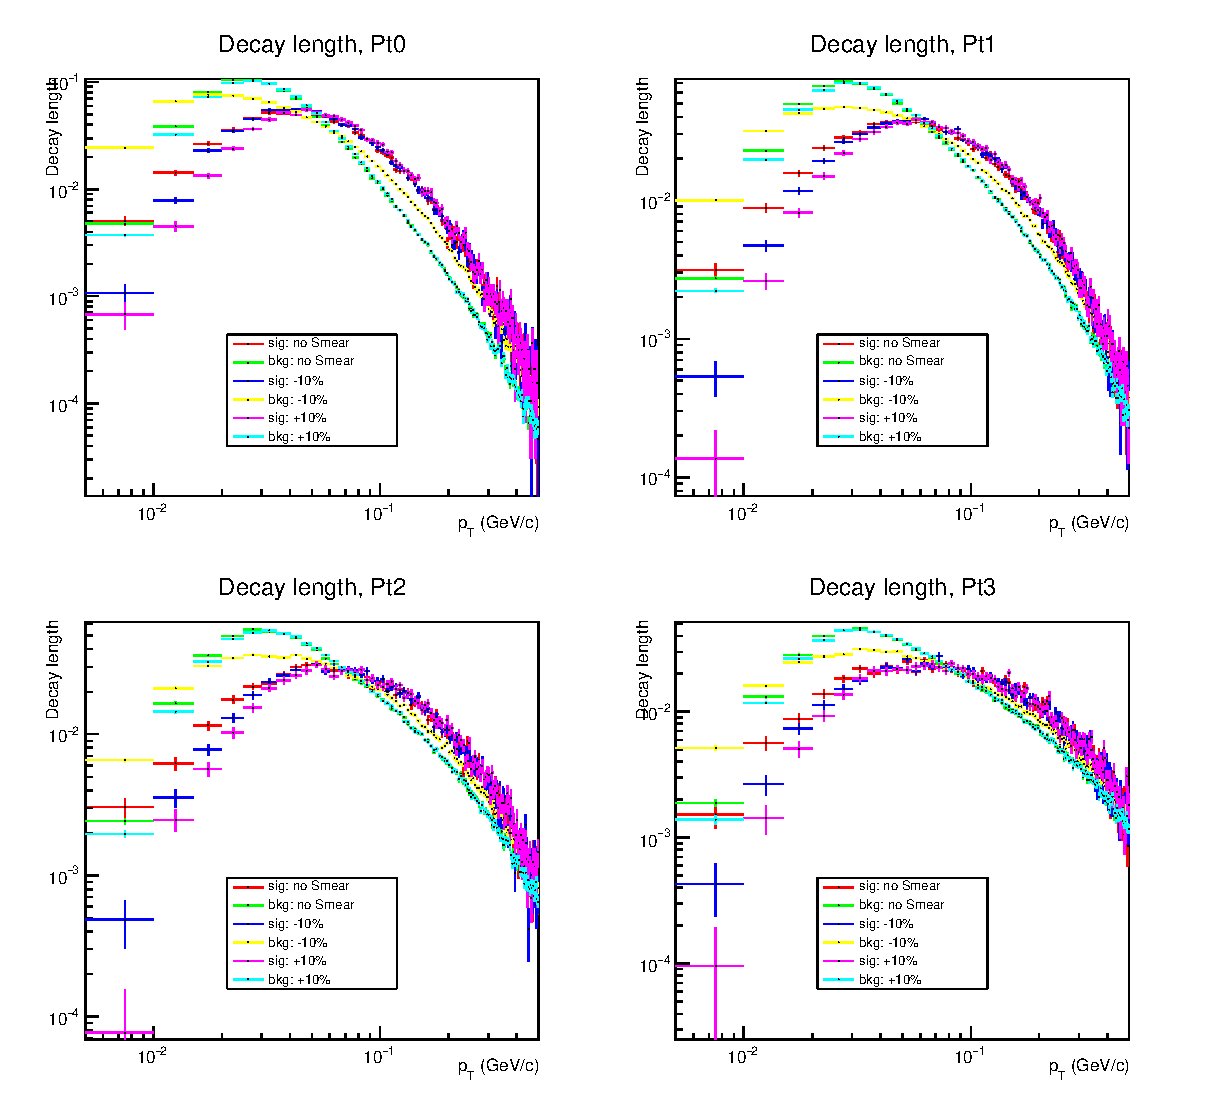
\includegraphics[width=.60\textwidth]{FigCap4/DL_smerp10m10.eps}
\caption{Decay length distribution w/o a 10\% applied smearing on xy impact parameter resolution, in different colours for signal and background.}             
\label{fig:DLwoSmear}
\end{center}
\end{figure}

\subsection{PID efficiency}
For the $\Ds$ a tigher PID selection was used in the analysis, and the test
without PID could not be carried out, due to the too low statistical 
significance obtained for the $\Ds$ without applying PID.
In the next subsections, the cases of the non strange D mesons and od $\Ds$ 
will be therefore discussed separately.

 The particle identification approach in the D meson 
 analysis consists in the evaluation of the compatibility
within $n\sigma$ from the expected dE/dx and time-of-flight 
values in a particular mass hypothesis. Usually,
in the D meson analysis, the systematic error on the PID is 
evaluated through the comparison of the
corrected yield obtained with and without applying the PID.
In the $\Ds$ case, the rare signal and the large background 
do not allow for a signal extraction without 
particle identification. The standard PID used for this meson 
(namely strong PID) was hence compared to the
standard one used for the non-strange D mesons (namely conservative PID).
 In Fig.~\ref{fig:rmsPID} it is shown the ratio
of the corrected yield obtained with conservative PID and the one 
obtained with the strong one, for the 12 different sets of cuts analysed.
The evaluation of this systematic was made considering only the
 third and fourth $\pt$ interval, as, in the other two intervals,
the yield extraction with conservative PID is problematic, due to 
the huge amount of background. The RMS of
the yield distribution in 6-8 and 8-12 GeV/c stays around 7\%, 
confirming the systematic uncertainty on PID quoted for the pass2 analysis.

\begin{figure}[!htb]
\begin{center}
 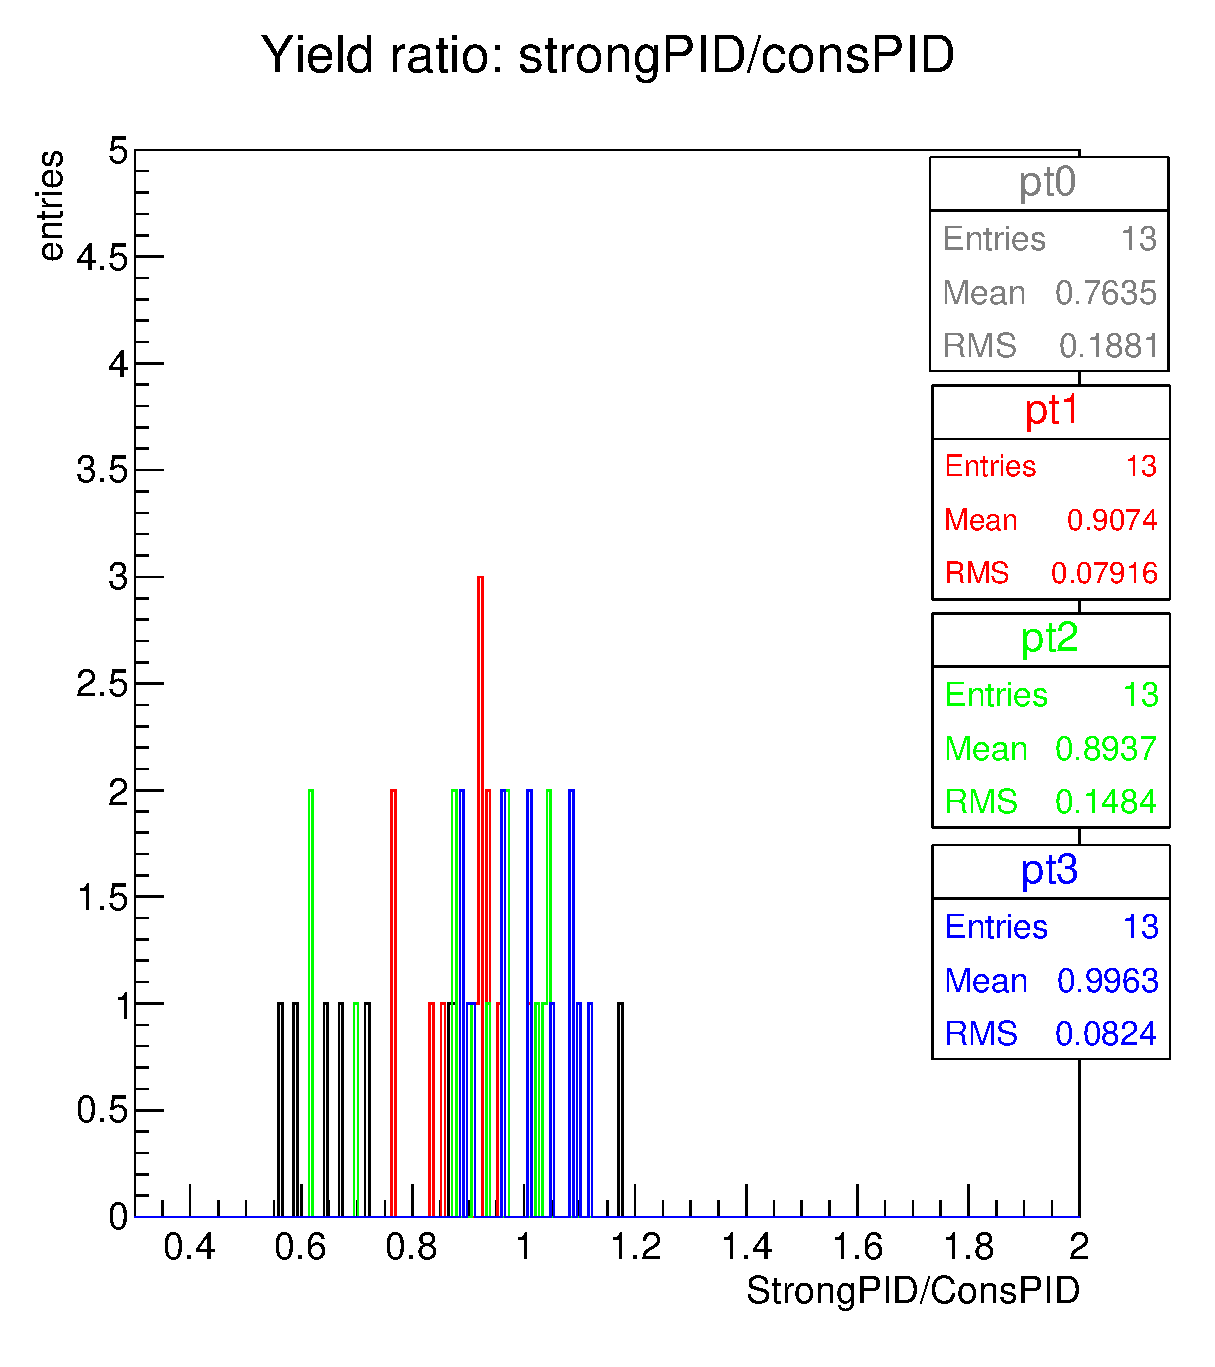
\includegraphics[width=.45\textwidth]{FigCap4/rms.eps}
\caption{Ratio of $\Ds$ corrected yield with 12 different sets of
cuts obtained with conservative and strong PID methods.}
\label{fig:rmsPID}
\end{center}
\end{figure}

\subsection{Track reconstruction efficiency}

The systematic uncertainty related to the tracking efficiency includes the 
effects arising from track finding in the TPC, from track propagation  
from the TPC to the ITS, and from track quality selections.
It was estimated with the following tests:
\begin{itemize}
\item comparison of the $\Dzero$ and $\Dplus$ cross sections obtained with different track selection cuts;
\item comparison of the TPC-ITS track matching efficiency in data and simulations.
\end{itemize}
These checks are discussed in detail in the following subsections.

\subsubsection{Variation of track selections}

The D-meson raw yields, efficiency and corrected yields were evaluated with 
different sets of track selection cuts.
Only one cut at a time was changed with respect to the standard values 
reported in Section?.
In particular, for the $\Dzero$ meson, the following four cut variations were 
tested:
\begin{enumerate}
\item additional cut on number TPC crossed rows $> 120-(5/\pt)$;
\item number of TPC clusters $>0.65 \times$ number of TPC crossed rows;
\item additional cut on number of clusters with TPC dE/dx signal $> 0.5 \times$ number of TPC crossed rows;
\item ratio of crossed rows over findable clusters in the TPC $>0.9$.
\end{enumerate}

The effect of the track cut variation on the raw yield, efficiency 
of prompt and feeddown $\Dzero$ mesons and on the prompt $\Dzero$ 
cross section are shown in Fig., where the ratios of 
the results obtained with the modified sets of track selections to those of 
the standard selection are reported.
The systematic uncertainty was assigned based on the observed variation of
the prompt $\Dzero$ cross section when varying the selections on the number of
TPC crossed rows and on the ratio of crossed rows over findable clusters.
The cut on the number of clusters with TPC dE/dx signal was not considered
for the estimation of the uncertainty since this selection is not applied
in the standard cuts.
 A systematic uncertainty of 2\% was therefore estimated due to track cut
variation.


In the $\Dplus$ case, the following four cut variations were tested:
\begin{enumerate}
\item additional cut on number TPC crossed rows $> 120-(5/\pt)$ (stc2);
\item number of TPC clusters $>0.65 \times$ number of TPC crossed rows (stc3);
\item ratio of crossed rows over findable clusters in the TPC $>0.9$ (stc4);
\item additional cut on the track geometric length (stc6). This was applied to 
the default values of SetCutGeoNcrNcl(3, 130, 1.5, 0.85, 0.7), where 3 is the 
width of the TPC dead zone, 130 is the cut on the geometrical length condition, 
1.5 is the 1/$\pt$ dependence slope, and 0.85 and 0.7 are the relative 
fractions of the cut conditions on Ncr and Ncl.
\end{enumerate}

The results are reported in fig., where the
top panel show the raw yield values extracted with the different set of cuts 
and the ratio to the standard cuts; the middle panel shows the efficiency for 
prompt $\Dplus$ mesons and the bottom panel the cross section.
The geometric length cut rejects 40--60\% of the signal (triplets of tracks):
this was expected because the efficiency of this cut is of about 80\% in a 
$\pt$ around 1 GeV/$c$, where there are most of the $\Dplus$ daughter tracks.
For the comparison of the cross section, one can see that a systematic 
deviation of about 3\% is observed when varying the cut on the ratio of 
crossed rows over findable clusters (stc4) and a trend with $\pt$ is observed 
in the deviation of the cross section when the additional $\pt$ dependent cut 
on the number of crossed rows is applied (stc2).
Based on these results, a 3\% systematic uncertainty was assigned.
Notice that this is larger than the 2\% effect observed for $\Dzero$ mesons,
reflecting the fact that $\Dplus$ are reconstructed from a three-body decay
channel, while $\Dzero$ from a two-prong decay.
For this reason, the 3\% uncertainty estimated with the $\Dplus$ was
assigned also to the $\Ds$ mesons, which are also reconstructed via a 
three-body decay and for which the lower statistical significance 
does not allow to estimate the systematic uncertainty with the same
precision obtained for the $\Dplus$.

\subsubsection{ITS-TPC matching efficiency}

Matching efficiency is defined as the fraction of tracks with 
clusters in both ITS and TPC over the total number of tracks with clusters in TPC.
Systematic uncertainty on its determination arises from discrepancies 
in efficiency between data and Monte Carlo.
Matching efficiency for primary tracks is expected to be higher than 
for secondary tracks (originating from strangeness decay, thus 
with secondary vertices likely to be out of SPD) or tracks arising
 from interaction with material.
If the fractions of primary and secondary tracks are different in data 
and in Monte Carlo, this could lead to a wrong estimation of systematic 
uncertainty in the matching. Hence, the idea here is to evaluate the
 real fraction of track types in data, and to use them to re-weight respective MC efficiencies 
to obtain a corrected inclusive MC efficiency. The latter will be compared 
with efficiency on data to extract the systematic uncertainty.\\
The ingredients are:
\begin{itemize}
\item Matching efficiencies for different particle types: 
Eff$^{\rm MC}_{\rm primaries}$, Eff$^{\rm MC}_{\rm secondaries}$, Eff$^{\rm Data}_{\rm inclusive}$
\item Fraction of primary tracks in data: f'$_{\rm primaries}$
\item Corrected MC-inclusive efficiency: 
Eff$^{\rm MC}_{\rm inclusive}$ = f'$_{\rm primaries}$ x Eff$^{\rm MC}_{\rm primaries}$ + (1- f'$_{\rm primaries}$) x Eff$^{\rm MC}_{\rm secondaries}$
\item Systematic uncertainty: 
(Eff$^{\rm Data}_{\rm inclusive}$ - Eff$^{\rm MC}_{\rm inclusive}$)/Eff$^{\rm Data}_{\rm inclusive}$
\end{itemize}
The same MC re-weighting procedure was already used in the 
charged-particle spectra analysis in pp at 5 TeV, with a slightly 
different algebra. Final results were checked to be in 
agreement with current analysis. \\
The Monte Carlo used here was the minimum bias 
LHC14j4b(c,d,e) anchored to LHC10b(c,d,e) pass4. 
Charm-enriched productions were rejected in this study as not
 advisable for fitting the DCA distribution at the level of the primary
  fraction extraction, since the peak shape of the DCA is slightly modified 
by the heavy flavour enrichment, making fit difficult to be performed. \\
Efficiency was studied as a function of:
\begin{itemize}
\item $\pt$, in 7 bins from 0.5 to 15 $\Gevc$
\item $\phi$, in 18 bins between (0,2$\pi$)
\item $\eta$, in 16 bins between (-0.8,0.8)
\end{itemize}

Let's examine below in detail the steps needed to 
calculate the systematic uncertainty.
\begin{enumerate}
\item {\bf ITS-TPC matching efficiency:} calculated separately for 
primary and secondary tracks in MC, inclusively on data. For the denominator
of the efficiency, i.e. tracks with TPC clusters, the selection was 
made requiring a TPC refit on the AliESDtracks, with no further 
requests on SPD clusters neither other ITS selections or refit. As 
for the numerator of the efficiency, the AliESDtracks were required 
to pass the kAny selection on SPD cluster, i.e. to have a cluster 
on at least one of the SPD layers. Tracks were selected requiring 
a cut on $|$DCAxy$|<$2.4 cm and on $|$DCAz$|<$3.2 cm.
\begin{figure}[!htb]
%\begin{center}
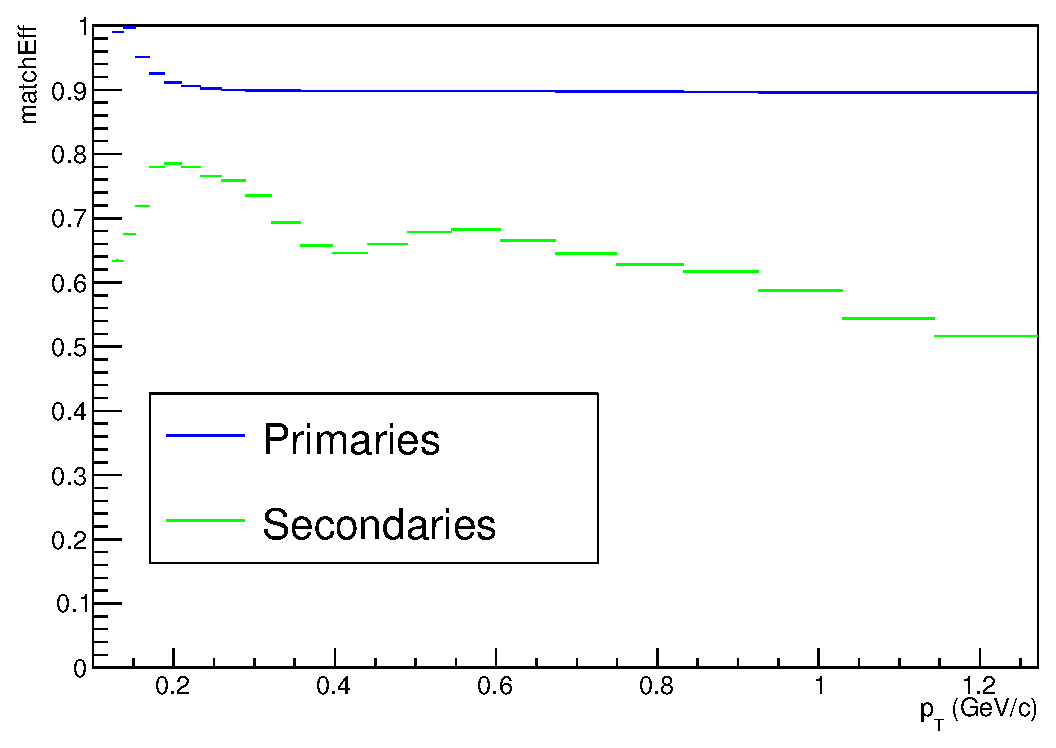
\includegraphics[height=5cm, width=7cm]{FigCap4/PT0_match_effprimsec.eps}
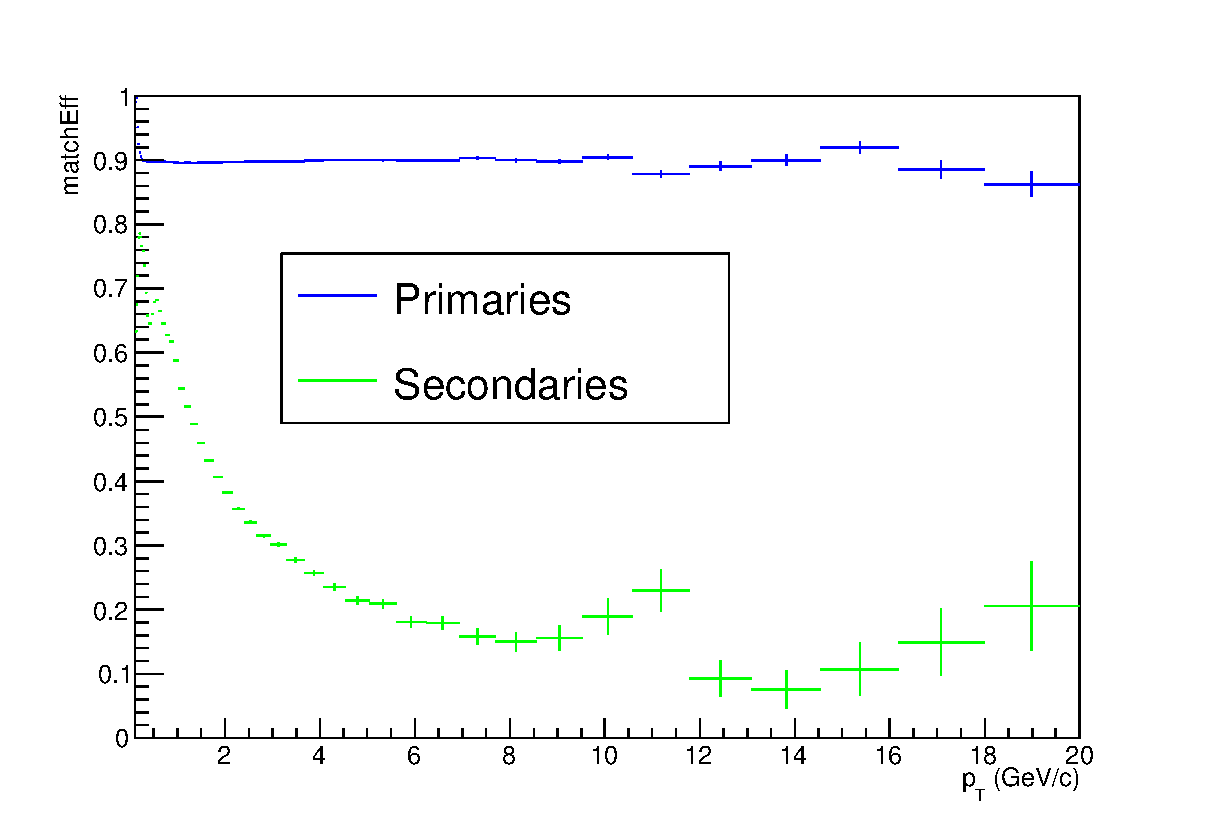
\includegraphics[height=5cm, width=7cm]{FigCap4/Allpt_matchingeff.eps}
\caption{Matching efficiency for primaries and secondaries tracks as a function of $\pt$ in MC sample related to  period b.  Left:  in $\pt$ intervals from 0. to 1 $\Gevc$. Right: in $\pt$ intervals from 0.5 to 20 $\Gevc$. }
\label{fig:matcheff_pt}
%\end{center}
\end{figure}
\begin{figure}[!htb]
\begin{center}
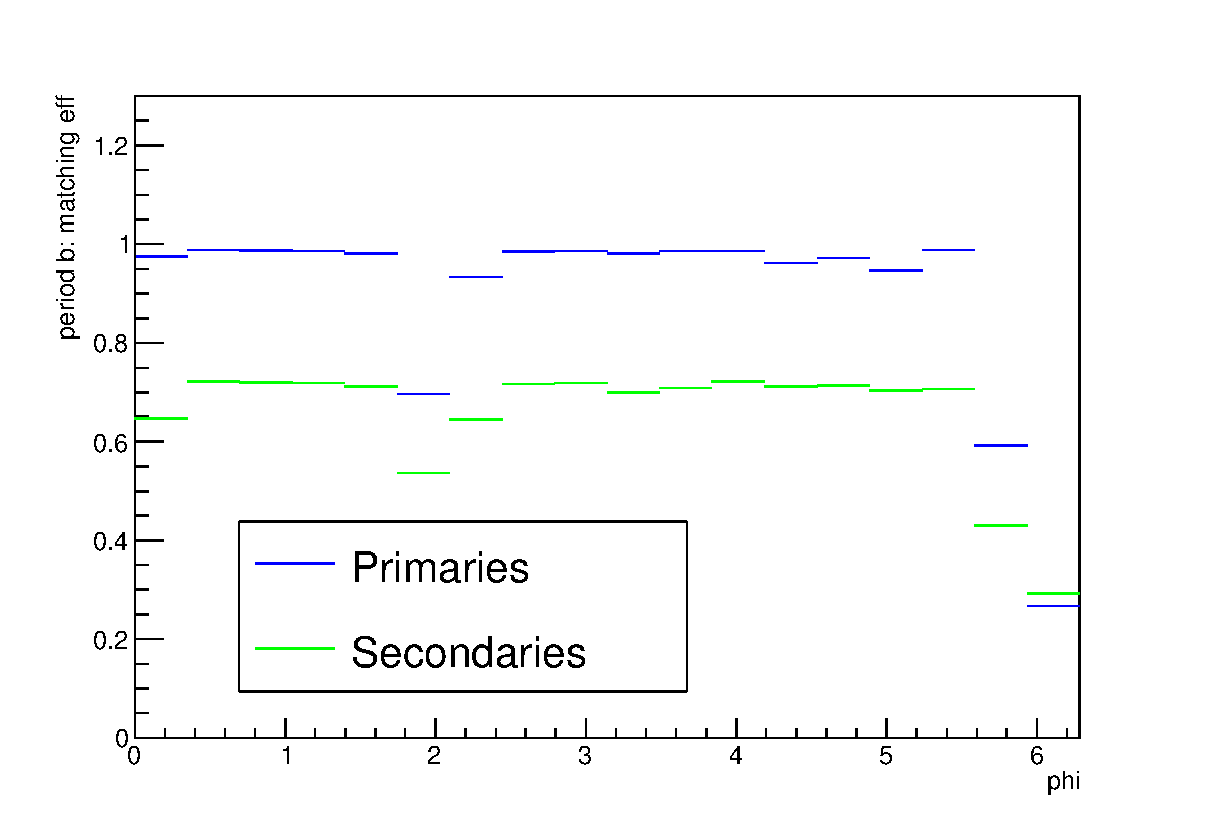
\includegraphics[width=.49\textwidth]{FigCap4/phi_allpt.eps}
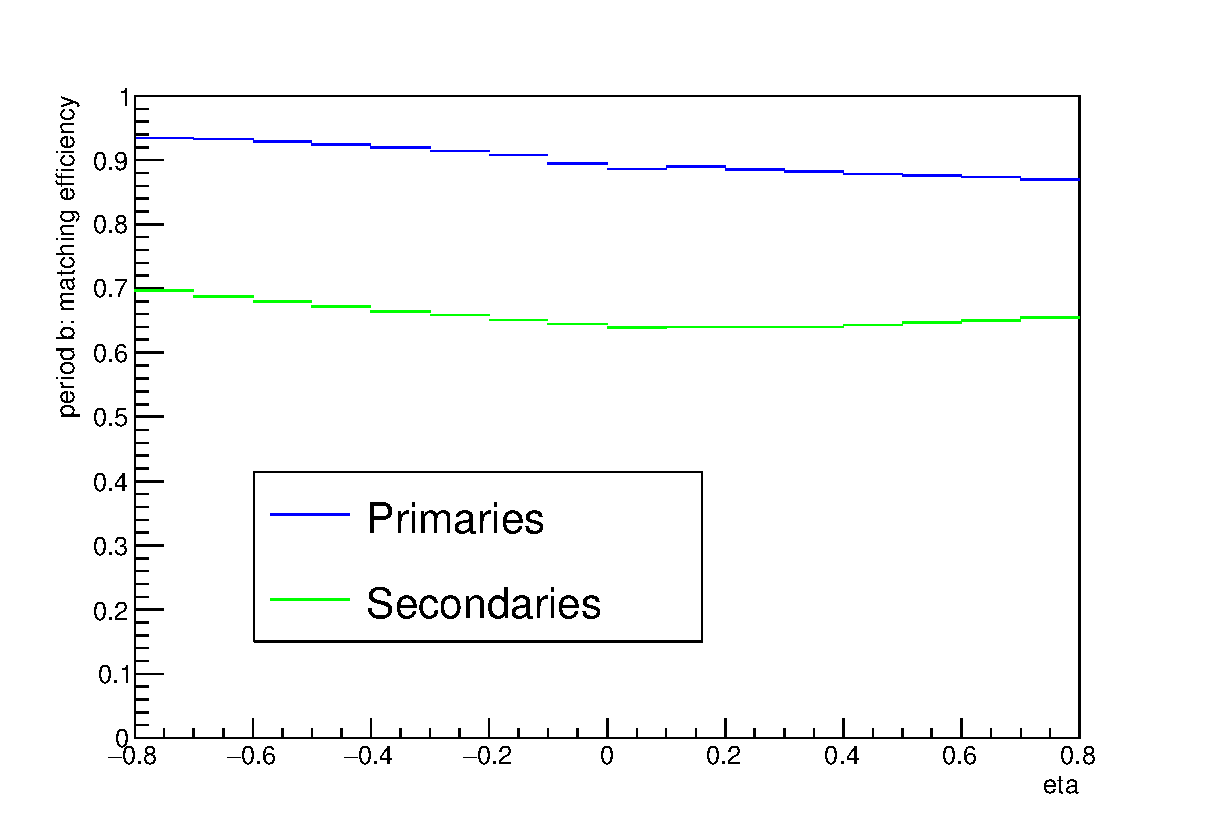
\includegraphics[width=.49\textwidth]{FigCap4/eta_range_matcheff.eps}
\caption{Matching efficiency for primaries and secondaries tracks in MC sample related to  period b.  Left:  as a function of $\phi$ in $\pt$ intervals from 0.5 to 14 $\Gevc$. Right: as a function of eta in $\pt$ intervals from 0.5 to 14 $\Gevc$. }
\label{fig:matcheff_phieta}
\end{center}
\end{figure}


In Fig.~\ref{fig:matcheff_pt}, matching efficiency as a function of 
$\pt$ is shown for the MC sample related to the period b of pass4 runs.  
The left panel  is referred to low $\pt$ (0-1 $\Gevc$), the right one
 to the range 0.5 to 20 $\Gevc$. 
In Fig.~\ref{fig:matcheff_phieta} matching efficiencies as a function of 
$\phi$ and $\eta$ are shown, in the $\pt$ range from 0.5 to 14 $\Gevc$.
 The trend of matching efficiency versus azimuthal angle $\phi$ clearly 
shows drops due to SPD inefficiencies during data taking.
\item {\bf Fractions of primary tracks:} extracted from a fit to
 the impact parameter distribution on data using MC templates for 
 primary and secondary contributions. The ROOT TFractionFitter 
 package was used to perform the fit. The fit could be resolved 
 using three templates describing primary particles, secondaries 
 from strangeness and secondaries from material. A selection on 
 tracks requiring SPD kAny was used, to assure enough resolution
  and distinguish primary from secondary DCA distributions.
Fit was performed on the DCAxy distributions of charged particles 
in the range [-1,1] cm, in different intervals of $\pt$, $\phi$, $\eta$ 
and constraining the 3 fractions within reasonable minimum and maximum values.
The fractions were then calculated integrating the histograms 
resulting from the fit in the range $|$DCAxy$|<$2.4 cm, for
consistency with matching efficiency calculation. In Fig.~\ref{fig:DCAxyDataMCVsPt}
 the distributions of DCAxy in data and in MC for the different contributions are
shown in different colours, in $\pt$ intervals from 0.5 to 15 $\Gevc$.
 In Fig.~\ref{fig:DCAxyRatioDataMCVsPt} the ratio of the distributions 
 of DCAxy in data and in MC (inclusive distribution) are also
shown in the same $\pt$ intervals of Fig.~\ref{fig:DCAxyDataMCVsPt}, 
while in Fig.~\ref{fig:DCAxyRatioDataFitVsPt} the ratio of the 
distributions of DCAxy in data with the fit-result histograms are plotted. 
In some $\pt$ intervals, for large DCAxy values, a quite large 
discrepancy data-MC template is observed.
Finally, in Fig.~\ref{fig:Fractions}, the primary and secondary
 fractions extracted from fit on data are shown and compared to 
 the ones obtained from MC truth (empty markers). As a closure test, 
 it was verified that the latter MC fractions did not change when extracting
them from a fit using TFractionFitter on MC inclusive distribution itself, 
with the three usual MC templates.  
The fraction of secondaries in the figure already includes contribution 
from material. We conclude that the fraction of secondaries is underestimated in MC.
\item {\bf Correction to the primary fraction:} since the fraction of primary
 particles was calculated on tracks passing the selection SPD kAny, we
need to rescale the primary fraction to the total number of tracks in TPC. 
The correction factor is based on MC information and obtained as 
the ratio of the fraction of primary tracks in TPC with the fraction of primary
 tracks with match TPC-ITS. The final fraction of primary tracks is hence
  f'$_{\rm primaries}$ = f$_{\rm primaries}$ x correction factor, 
  where f$_{\rm primaries}$ is the fraction obtained at step 2. 
  Typical values of correction factor are around $\sim$ 0.95-0.98. 
  In Fig.~\ref{fig:MCfractions} an example of fractions of primary 
  and secondary tracks in MC requiring ITS-TPC or TPC only are 
  shown in different colours as a function of $\pt$.

\item {\bf ITS-TPC corrected matching efficiency:} calculated 
as  Eff$^{\rm MC}_{\rm inclusive}$ = f'$_{\rm primaries}$ x Eff$^{\rm MC}_{\rm primaries}$ + (1- f'$_{\rm primaries}$) x Eff$^{\rm MC}_{\rm secondaries}$. The corrected matching efficiency 
is shown in Fig.~\ref{fig:CorrMatchEffVsPt},~\ref{fig:CorrMatchEffVsPhi}, 
as a function of $\pt$, $\phi$, $\eta$ respectively, for kaons and 
pions only (using particle identification, requiring a 3-sigma cut). 
It was verified that no substantial changes are obtained if 
considering all the species (pions, kaons, protons, electrons, muons). 
Finally, the ratios of the latter inclusive MC-corrected efficiencies with
 data are shown in Fig.~\ref{fig:SysMatchEffVsPt},~\ref{fig:SysMatchEffVsPhi},~\ref{fig:SysMatchEffVsEta}. 
 It is evident how the re-weighting of MC with the real fractions 
of track types is useful in quoting a truthful and reduced systematic uncertainty. \\ 
Error bars were assigned to matching efficiency to account for statistical fluctuations.
A final systematic uncertainty of 2\% per track is assigned for particles 
between 2-6 $\Gevc$, and of 1\% at lower and higher $\pt$.
This per-track uncertainty needs to be summed in quadrature with the 
1\% uncertainty coming from systematic on track selection. \\
Finally, a MC simulation was used to propagate the uncertainty at the 
track level to the D meson level, accounting for the daughter's 
kinematic in the D-meson $\pt$ range of our analysis. In the MC 
simulation the same topological and PID cuts used on data were 
applied, to account also for possible influence of topological selection
 on daughter's kinematics. In the left column of 
 Fig.?, one can see the 
scatter plot of D-meson $\pt$ versus daughter's $\pt$ 
(for $\Dplus$, $\Ds$ and $\Dzero$ from top to bottom). 
The right column shows instead the final systematic on matching
 efficiency we quote for 2- and 3-prong D mesons as a function of $\pt$.
\end{enumerate}

\begin{figure}[!htb]
\begin{center}
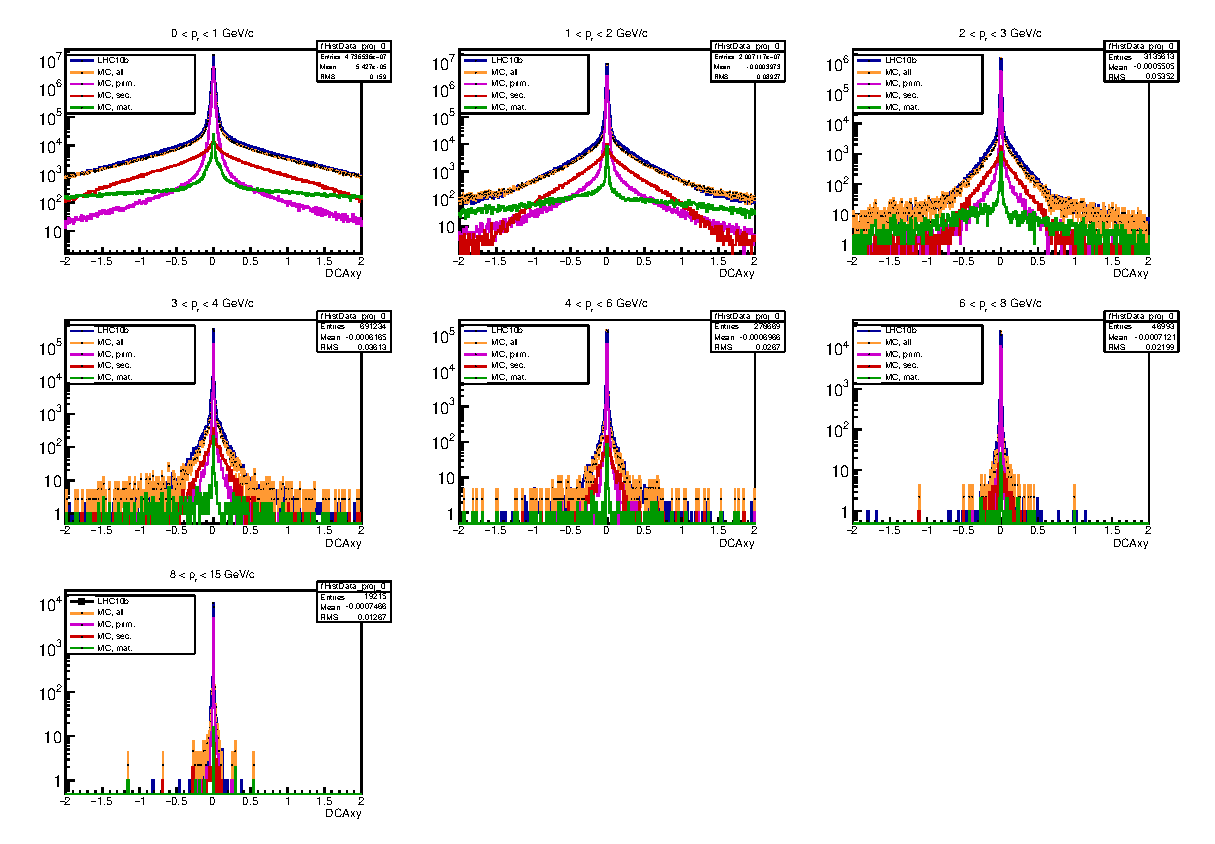
\includegraphics[width=.99\textwidth]{FigCap4/components_b_VsPt.eps}
\caption{DCAxy distributions in data and in MC for primary and secondary tracks in different colours, in $\pt$ intervals from 0.5 to 15 $\Gevc$.}
\label{fig:DCAxyDataMCVsPt}
\end{center}
\end{figure}

\begin{figure}[!htb]
\begin{center}
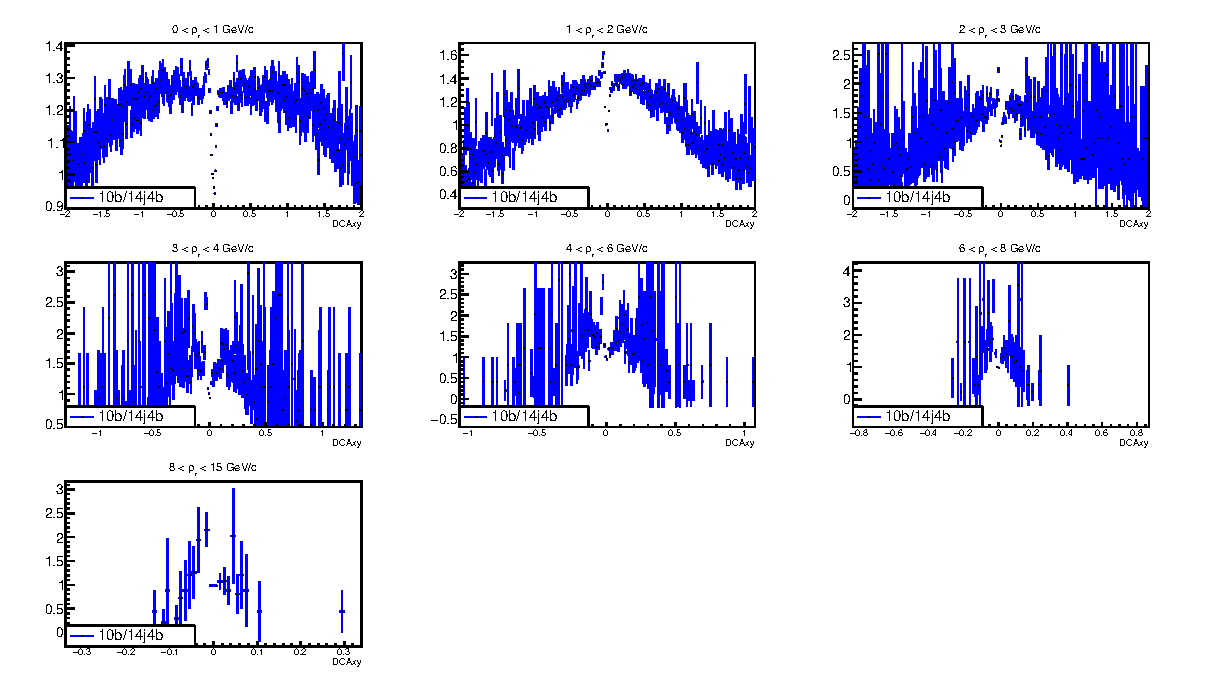
\includegraphics[width=.99\textwidth]{FigCap4/ratioDataMC_b_VsPt.eps}
\caption{Ratio of DCAxy distributions in data and in MC (inclusive distribution), in $\pt$ intervals from 0.5 to 15 $\Gevc$.}
\label{fig:DCAxyRatioDataMCVsPt}
\end{center}
\end{figure}

\begin{figure}[!htb]
\begin{center}
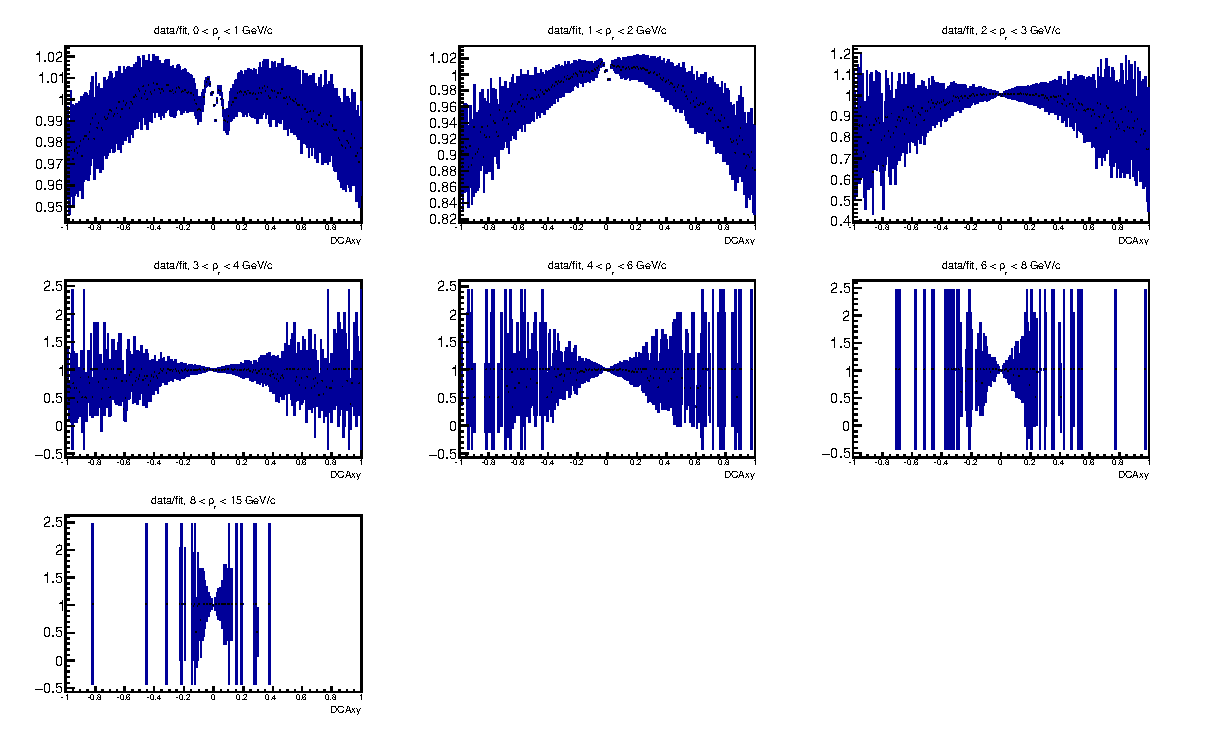
\includegraphics[width=.99\textwidth]{FigCap4/ratioDataFit_b_VsPt.eps}
\caption{Ratio of DCAxy distributions in data and in the fit result histograms, in $\pt$ intervals from 0.5 to 15 $\Gevc$.}
\label{fig:DCAxyRatioDataFitVsPt}
\end{center}
\end{figure}

\begin{figure}[!htb]
\begin{center}
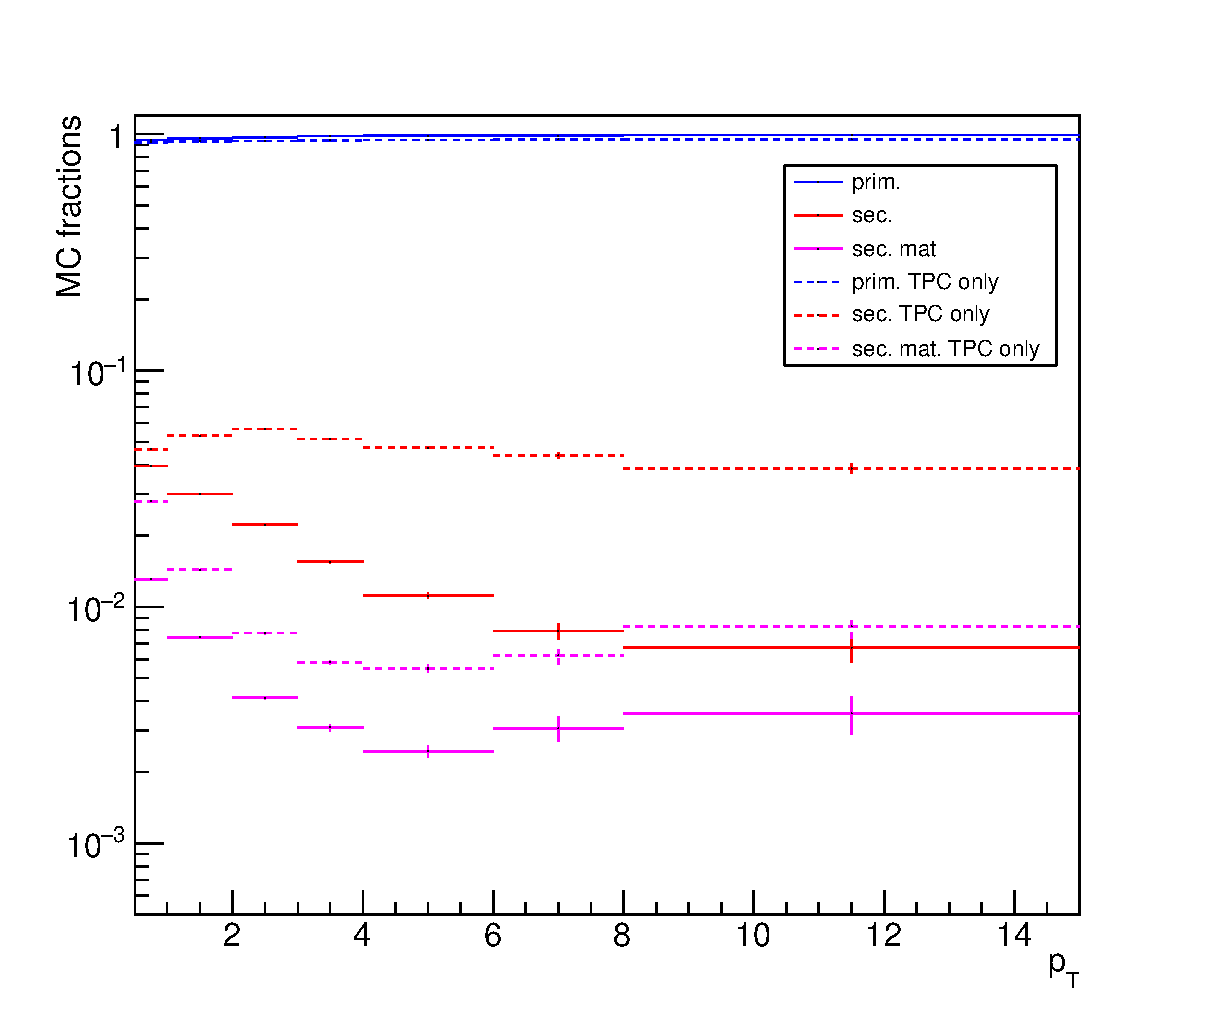
\includegraphics[width=.50\textwidth]{FigCap4/MCfractions_KaonPion_ESDTrOnly_b_VsPt.eps}
\caption{Example of fractions of primary and secondary tracks in MC requiring ITS-TPC or TPC only in different colours as a function of $\pt$.}
\label{fig:MCfractions}
\end{center}
\end{figure}

\begin{figure}[!htb]
\begin{center}
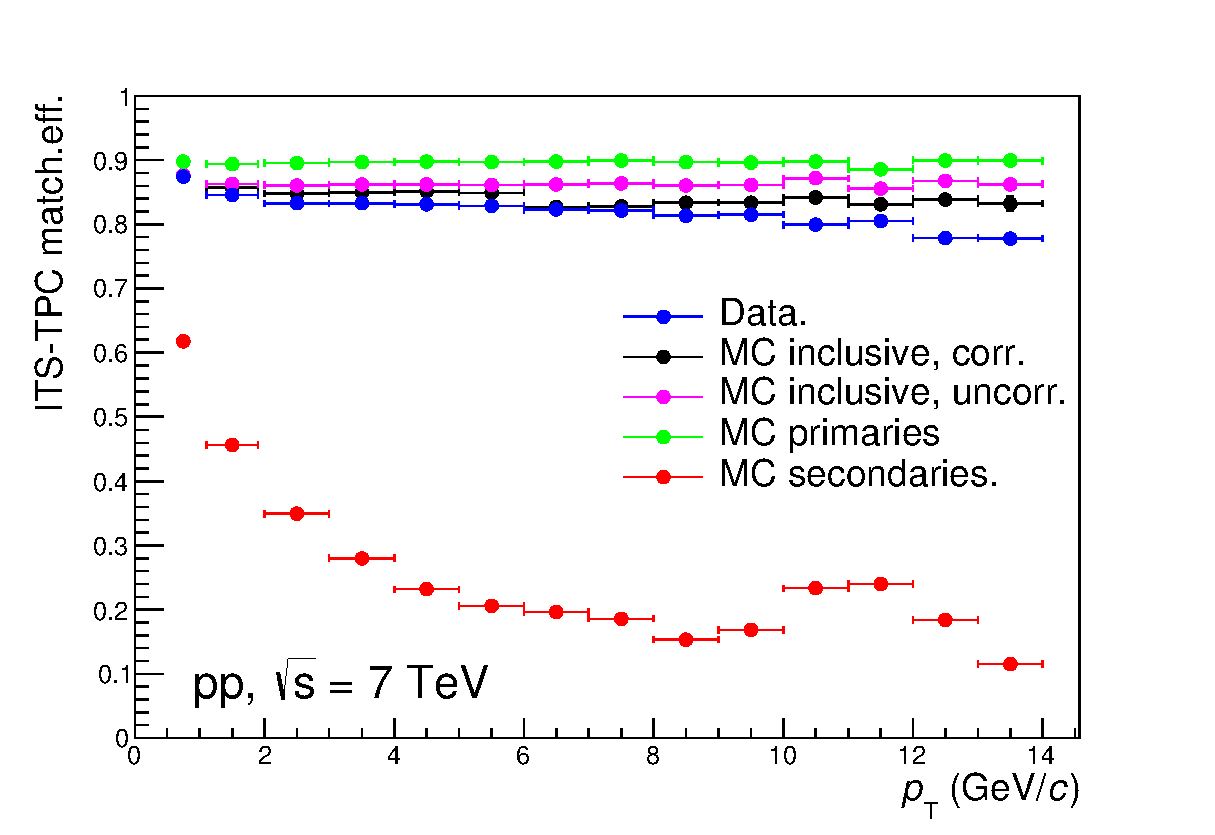
\includegraphics[height=7cm]{FigCap4/ITSTPCmatchEff_10bpass4_vsPt.eps}
\caption{Matching Efficiency as a function of $\pt$ for period b (left), and period d (right). The matching efficiency is shown for data (blu) for MC primaries and secondaries, separately (green and red), and for the MC corrected with the fraction of secondaries and primaries (black) Also the uncorrected MC is shown (magenta). }
\label{fig:CorrMatchEffVsPt}
\end{center}
\end{figure}

\begin{figure}[!htb]
\begin{center}
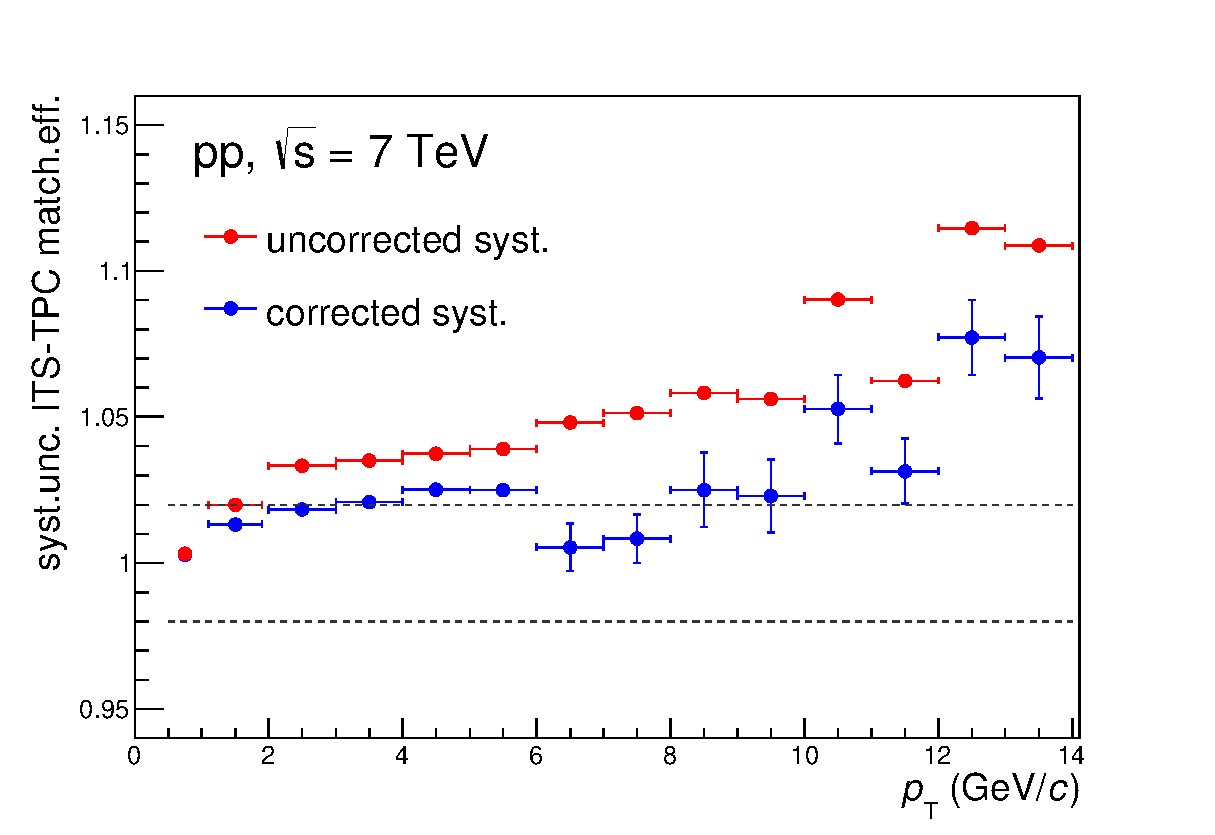
\includegraphics[height=7cm]{FigCap4/ITSTPCmatchEffSyst_10bpass4_vsPt.eps}
\caption{Matching Efficiency as a function of $\pt$ for period b (left), and period d (right). The matching efficiency is shown for data (blu) for MC primaries and secondaries, separately (green and red), and for the MC corrected with the fraction of secondaries and primaries (black) Also the uncorrected MC is shown (magenta). }
\label{fig:CorrMatchEffVsPt}
\end{center}
\end{figure}

\begin{figure}[!htb]
\begin{center}
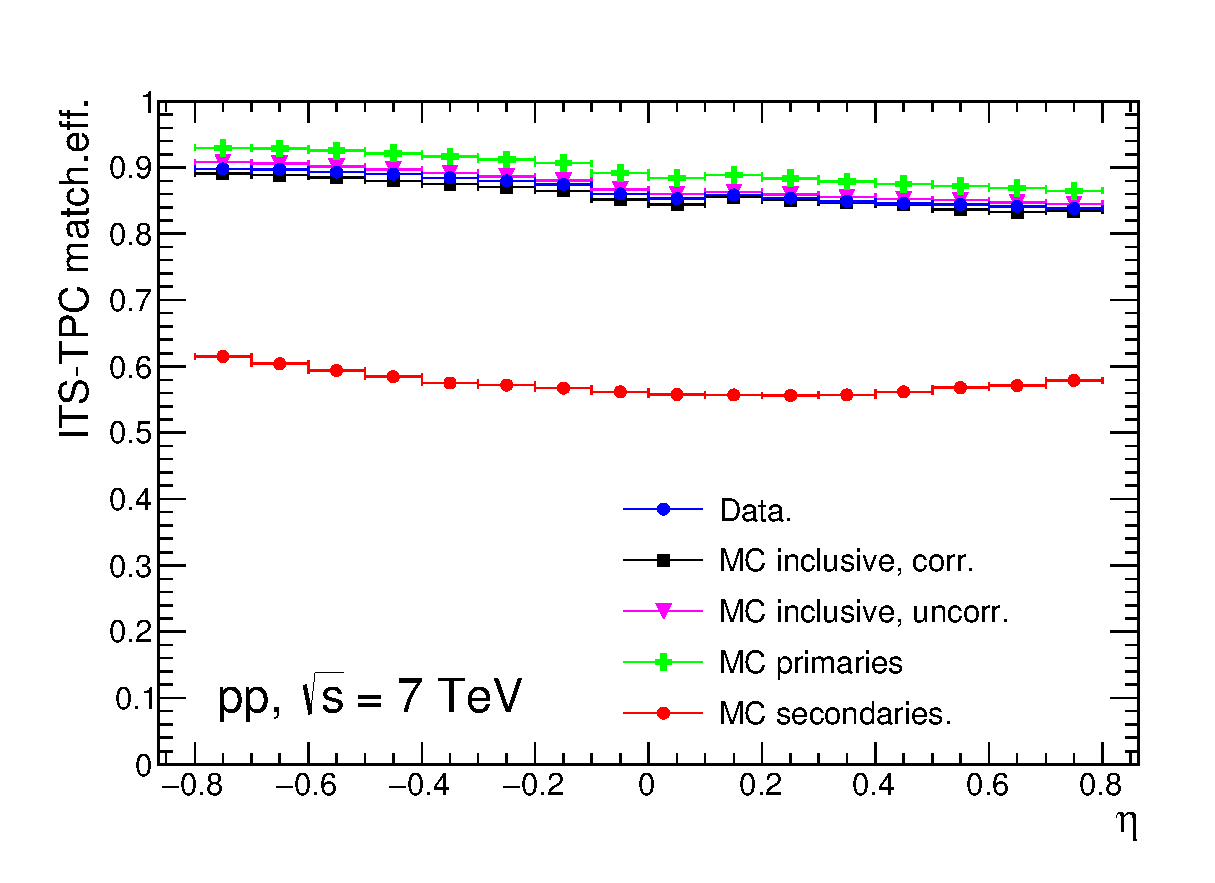
\includegraphics[width=.49\textwidth]{FigCap4/ITSTPCmatchEff_10bpass4_vsEta.eps}
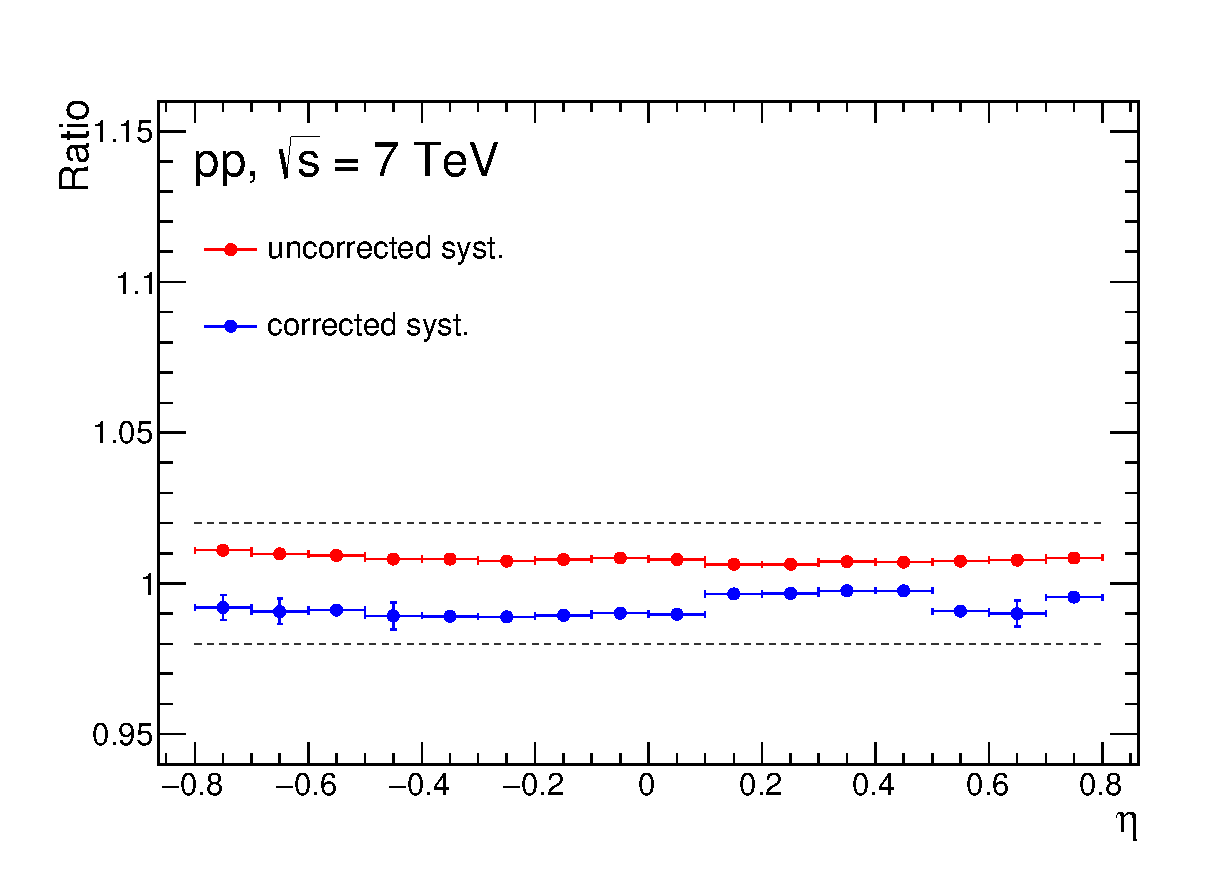
\includegraphics[width=.49\textwidth]{FigCap4/ITSTPCmatchEffSyst_10bpass4_vsEta.eps}
\caption{Matching Efficiency as a function of $\pt$ for period b (left), and period d (right). The matching efficiency is shown for data (blu) for MC primaries and secondaries, separately (green and red), and for the MC corrected with the fraction of secondaries and primaries (black) Also the uncorrected MC is shown (magenta). }
\label{fig:CorrMatchEffVsEta}
\end{center}
\end{figure}

\begin{figure}[!htb]
\begin{center}
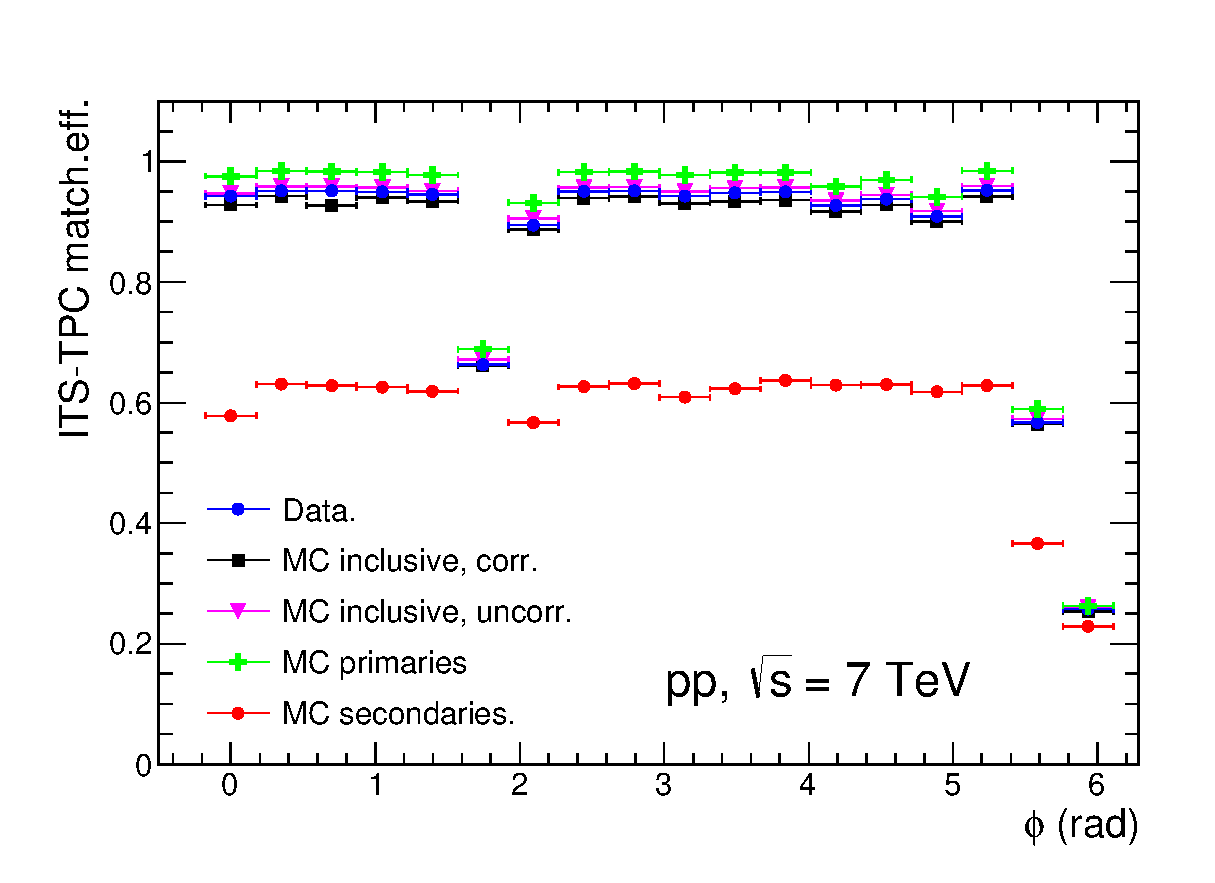
\includegraphics[width=.49\textwidth]{FigCap4/ITSTPCmatchEff_10bpass4_vsPhi.eps}
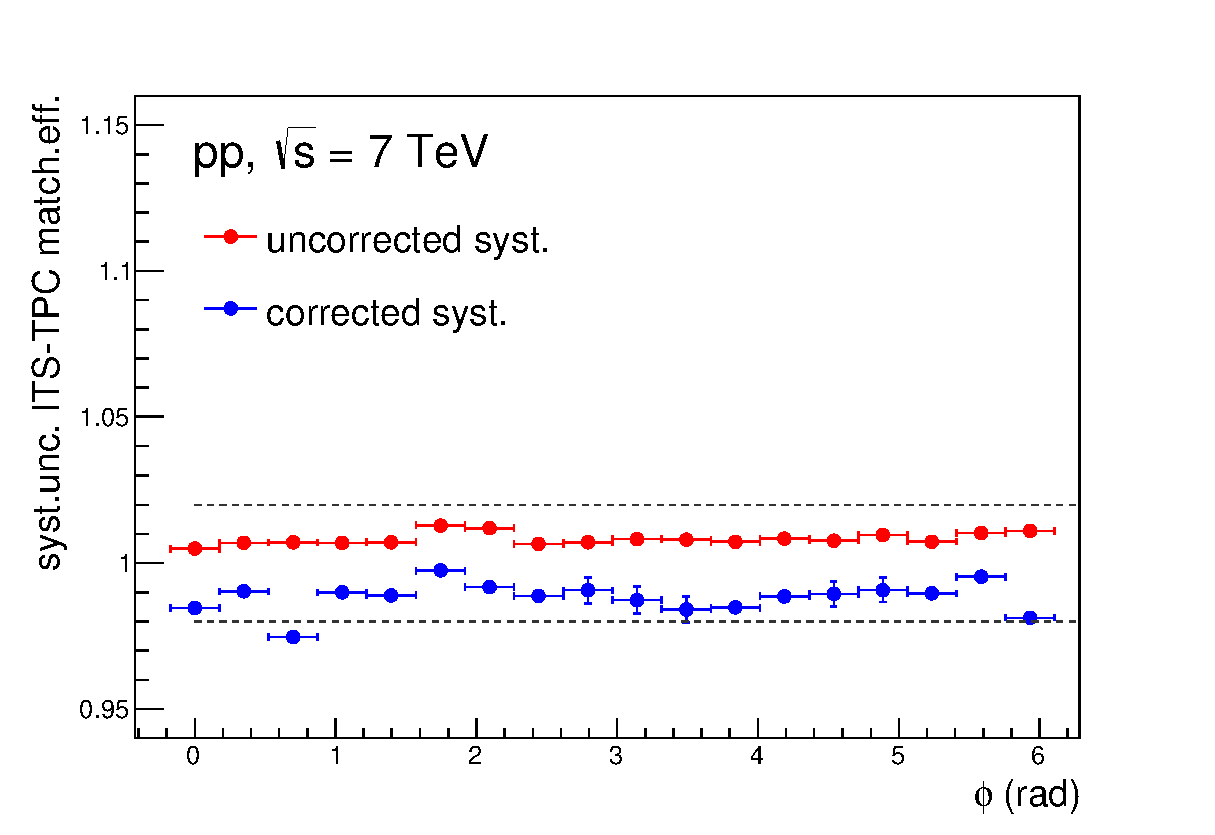
\includegraphics[width=.49\textwidth]{FigCap4/ITSTPCmatchEffSyst_10bpass4_vsPhi.eps}
\caption{Matching Efficiency as a function of $\pt$ for period b (left), and period d (right). The matching efficiency is shown for data (blu) for MC primaries and secondaries, separately (green and red), and for the MC corrected with the fraction of secondaries and primaries (black) Also the uncorrected MC is shown (magenta). }
\label{fig:CorrMatchEffVsPhi}
\end{center}
\end{figure}

\begin{figure}[!htb]
\begin{center}
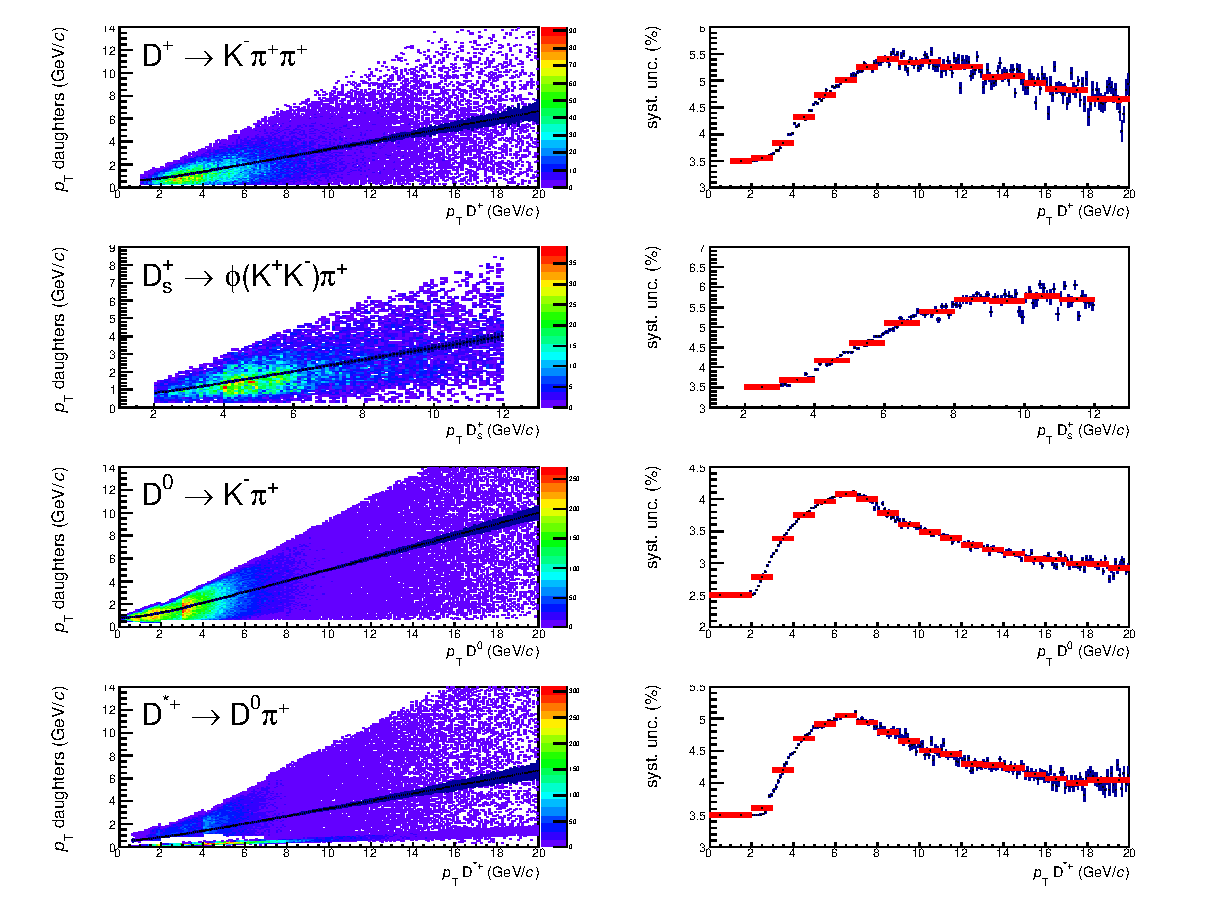
\includegraphics[width=1\textwidth]{FigCap4/FinalSystMEDmesons_ppPass4.eps}
\caption{Left column: scatter plot of daughter's $\pt$ versus D-meson $\pt$ for $\Dplus$, $\Ds$, $\Dzero$ and $\Dstar$ from top to bottom. Right column: final systematic uncertainties propagated at D-meson level after weighting for daughter's kinematics, as a function of $\pt$.}
\label{fig:SysMatchEffVsPhi}
\end{center}
\end{figure}

\subsection{B feed-down}
In the framework of D-meson analysis we currently use two different 
methods for the B feed-down subtraction, namely N$_{\rm b}$ and $f_{\rm c}$. 
The first method, used to give the central value for $f_{\rm prompt}$, 
needs as inputs for the calculations the FONLL predictions
for B-meson cross-sections and the Monte Carlo efficiency for B feed-down 
D mesons.
The second method, instead, takes as inputs FONLL predictions for both 
feed-down and prompt D mesons and their respective Monte Carlo efficiencies, 
as follows:\\
\begin{equation}
f^\prime_{\rm prompt} = \left( 	1 + 	\frac{({\rm Acc}\times\epsilon)_{{\rm feed-down}}}{({\rm Acc}\times\epsilon)_{{\rm prompt}}}	\cdot
		 \frac{ \left(\frac{{\rm d}^2 \sigma}{{\rm d}y \, {\rm d} \pt } \right)^{{\sf FONLL}}_{{\rm feed-down}} }{ \left(\frac{{\rm d}^2 \sigma}{{\rm d}y \, {\rm d} \pt } \right)^{{\sf FONLL}}_{ {\rm prompt} } } 
\right)^{-1} \, .
\label{eq:fc}
\end{equation}
\\We want to compare now FONLL predictions for heavy-flavored hadrons
 to the current available measurements of beauty and charmed 
 meson cross-sections at the LHC.
It is useful in order to decide whether to continue with the 
double-method strategy or to reduce to the N$_{b}$-only usage.
In Fig.~\ref{fig:Bmesons} the B$^{+}$, B$^{0}$, B$_{\rm s}$ and 
$\Lambda_{\rm b}$ cross-sections measured by CMS in pp collisions at 7 TeV
are compared with FONLL predictions.
The measurements lay within FONLL uncertainty bands in the case 
of non-strange B mesons. 
In Fig.~\ref{fig:LHCbBmesons}, measurements of B hadrons from 
LHCb in pp collisions at 7 TeV in the rapidity interval 
\mbox{2.0 $< y_{\rm cm} <$ 4.5}  are shown.
To scale FONLL predictions we used the fragmentation fraction values 
of b quarks into B hadrons measured by LHCb in the rapidity interval 
2.0 $< y_{\rm cm} <$ 4.5. Such measurements aim for an 
enhancement of bayon production at high rapidity with respect to 
mid-rapidity, in spite of a decrease of non-strange B-meson production. 
In Fig.~\ref{fig:LHCbBmesons}, starting from the top left figure, the 
comparison between LHCb B$^{+}$-meson cross-section and FONLL
 curve shows good agreement.
The top right plot shows instead a better agreement for 
B$_{\rm s}$-meson data from LHCb with FONLL, in a wider 
$p_{T}$ range than those of CMS.
The CMS and LHCb B$_{\rm s}$-meson cross-sections in 
8 $< p_{\rm T} <$ 50 GeV/$c$ as a function of y are shown in 
the bottom left plot, together with the FONLL predictions in the 
two different rapidity intervals. For the CMS data, two cases are 
reported, one obtained using the current (2015) PDG value for 
BR(B$_{\rm s} \rightarrow J/{\rm \psi} ~\Phi$),
the other obtained using the 2010 PDG value, referenced in the 
CMS paper. As regards $\Lambda_{\rm b}$ cross-section 
(bottom right plot), FONLL provides a shape which is compatible
 with LHCb data, provided a rescaling of a factor 2, which may account
  for uncertainties on the determination of the BR($\Lambda_{b} \rightarrow J/\psi {\rm p K}$) 
  used by LHCb to provide the cross-section.
In Fig.~\ref{fig:Dmesons} we can see the $J/\psi$ from beauty-decay 
cross-section in pp collisions at 7 TeV measured by LHCb, and the 
D$^{+}$-, D$^{0}$-, D$^{*+}$-meson cross-sections at 7 TeV by ALICE.
In the case of $J/\psi$ meson, FONLL provides a good description of 
the 7 TeV data, as well as for the 8 TeV ones (not shown here). 
The D-meson results show that 
experimental data sistematically lay on the upper edge of FONLL uncertainty 
band, thus charm production being underestimated by FONLL.\\
Considering that:
\begin{itemize}
\item FONLL provides a good description of B$^{+}$-, B$^{0}$-meson 
cross-sections at 7 TeV both at mid- and forward rapidity and of 
$J/{\rm \psi}$-meson cross-section at forward rapidity;
\item FONLL provides a good description also for the 
B$_{\rm s}$-meson and $\Lambda_{\rm b}$-baryon cross-sections 
at forward rapidity where data are available in a wider $p_{T}$ range 
than at mid-rapidity, allowing for a safer comparison. The rescaling 
of the shape for the $\Lambda_{\rm b}$ cross-section could be due 
to the uncertainty on the branching ratio
of the channel used by LHCb in the analysis,
\end{itemize}
the calculation of $f_{\rm prompt}$ with the $N_{\rm b}$ method is then fully justified.
The $f_{\rm c}$ method, instead, would suffer from the 
underestimation of charm production at the
LHC energies. It is reasonable to conclude, thanks to the available 
measurements, that $f_{\rm c}$ would artificially introduce a bias if 
used to subtract the beauty feed-down component.
Besides, this choice will give benefit to our feed-down systematic 
estimate. In Tab.~\ref{tab:systFD} we can see an example for the D$_{\rm s}$.

\begin{table}[tbh!]
\centering
\begin{tabular}{|clc|c|c|c|} 
\hline
& \multicolumn{2}{c|}{N$_{\rm b}$ + $f_{\rm c}$} & \multicolumn{2}{c|}{N$_{\rm b}$ only}\\
\hline
$p_{\rm T}$ (GeV/c) & +systFD & -systFD & +systFD & -systFD \\
\hline
2-4        & 4.1\% & 17.0\% & 4.1\% & 4.6\%\\
4-6        & 3.7\% & 10.2\% & 3.7\% & 4.7\%\\
6-8        & 3.8\% & 10.0\% & 3.8\% & 4.8\%\\
8-12        & 4.0\% & 9.0\% & 4.0\% & 4.8\%\\
\hline
\end{tabular}
\caption{Comparison of the systematic uncertainty on the feed-down subtraction for the D$_{\rm s}$ meson.} 
\label{tab:systFD}
\end{table}

\subsection{Generated $\pt$ shape}

The systematic effect on the efficiency extracted from the simulations due to
the generated $\pt$ shape of D mesons was tested by computing the efficiency
with and without using in the AliCFTaskVertexingHF task the $\pt$-dependent 
weights  that allow us to correct for the difference between the $\pt$ 
spectrum of generated $\Dzero$ mesons in the LHC10f7a production and the 
prediction from FONLL.


\begin{table}[!tb]
\centering
\begin{tabular}{l|ccccc|}
 \hline 
  & \multicolumn{4}{c|}{$\pt$ interval ($\GeV/c$)}\\
 & 2--4 & 4--6 & 6--8 & 8--12\\
\hline
Raw yield extraction & 5\%& 5\%& 5\%& 5\%\\
Topol. sel. efficiency & 7\%& 7\%& 7\%& 7\%\\
Tracking efficiency & 5\%& 5.5\% & 6\% & 6\%\\
PID efficiency & 7\%& 7\%& 7\%& 7\%\\
MC $\pt$ shape   &3\%&3\%&2\%&2\%\\
Feed-down from B & $^{+4.1\%}_{-4.6\%}$& $^{+3.7\%}_{-4.7\%}$& $^{+3.8\%}_{-4.8\%}$& $^{+4.0\%}_{-4.8\%}$\\
Luminosity  
  & \multicolumn{4}{c|}{3.5\%} \\
\hline 
\end{tabular}
\caption{Relative systematic uncertainties on the $\pt$-differential production
cross section of prompt $\Ds$ mesons.}
\label{tab:SystDs}
\end{table}

\section{Results}
The $\pt$-differential cross sections for prompt D-meson production
are reported in this section.
In Fig., the $\Dzero$-meson cross section
from this analysis is compared to the published one based on the analysis of 
the pass2 reconstruction of the 2010 pp sample and to FONLL calculations.
The ratios to FONLL predictions for the new and the published analyses
and of the new result to the published one are also reported.
The comparison of the relative statistical and systematic uncertainties
on the new and on the published (pass2) results are shown in 
Fig..
The statistical uncertainties on the new results are slightly reduced as
compared to the published one, while there is a substantial reduction, 
by a factor 1.5--3 depending on $\pt$, of the systematic uncertainties.



The $\Ds$-meson $\pt$-differential cross sections are shown in 
Fig.~\ref{fig:CrossSecDs2vs4}, where they are compared to the
published results based on the pass2 reconstruction.
The comparison to the predictions from pQCD calculations with the
GM-VFNS approach and the LO $k_{\rm T}$ factorization 
algorithm are shown in Fig.~\ref{fig:CrossSecDsvsGMVFNS}.


\begin{figure}[!htb]
\begin{center}
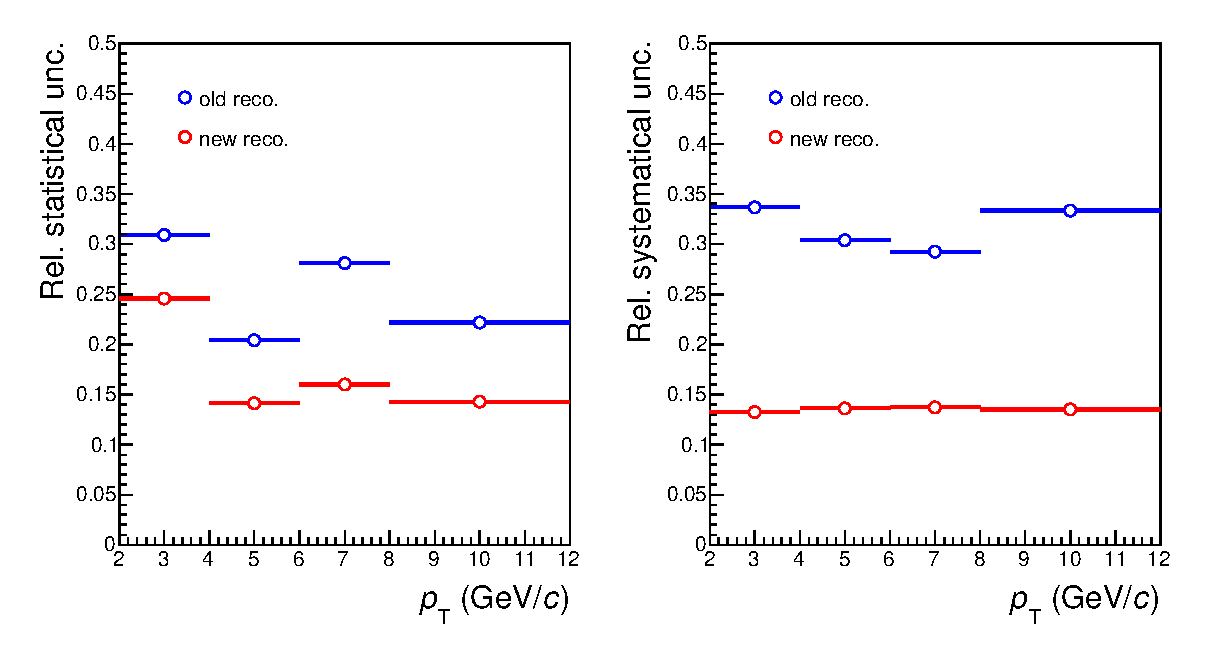
\includegraphics[width=.99\textwidth]{FigCap4/uncertainties_pass2_pass4.eps}
\caption{Comparison of statistical and systematic uncertainty on $\Ds$-meson
cross section in the pass2-based publication and this re-analysis.}
\label{fig:CrossSecDs2vs4}
\end{center}
\end{figure}

\begin{figure}[!htb]
\begin{center}
%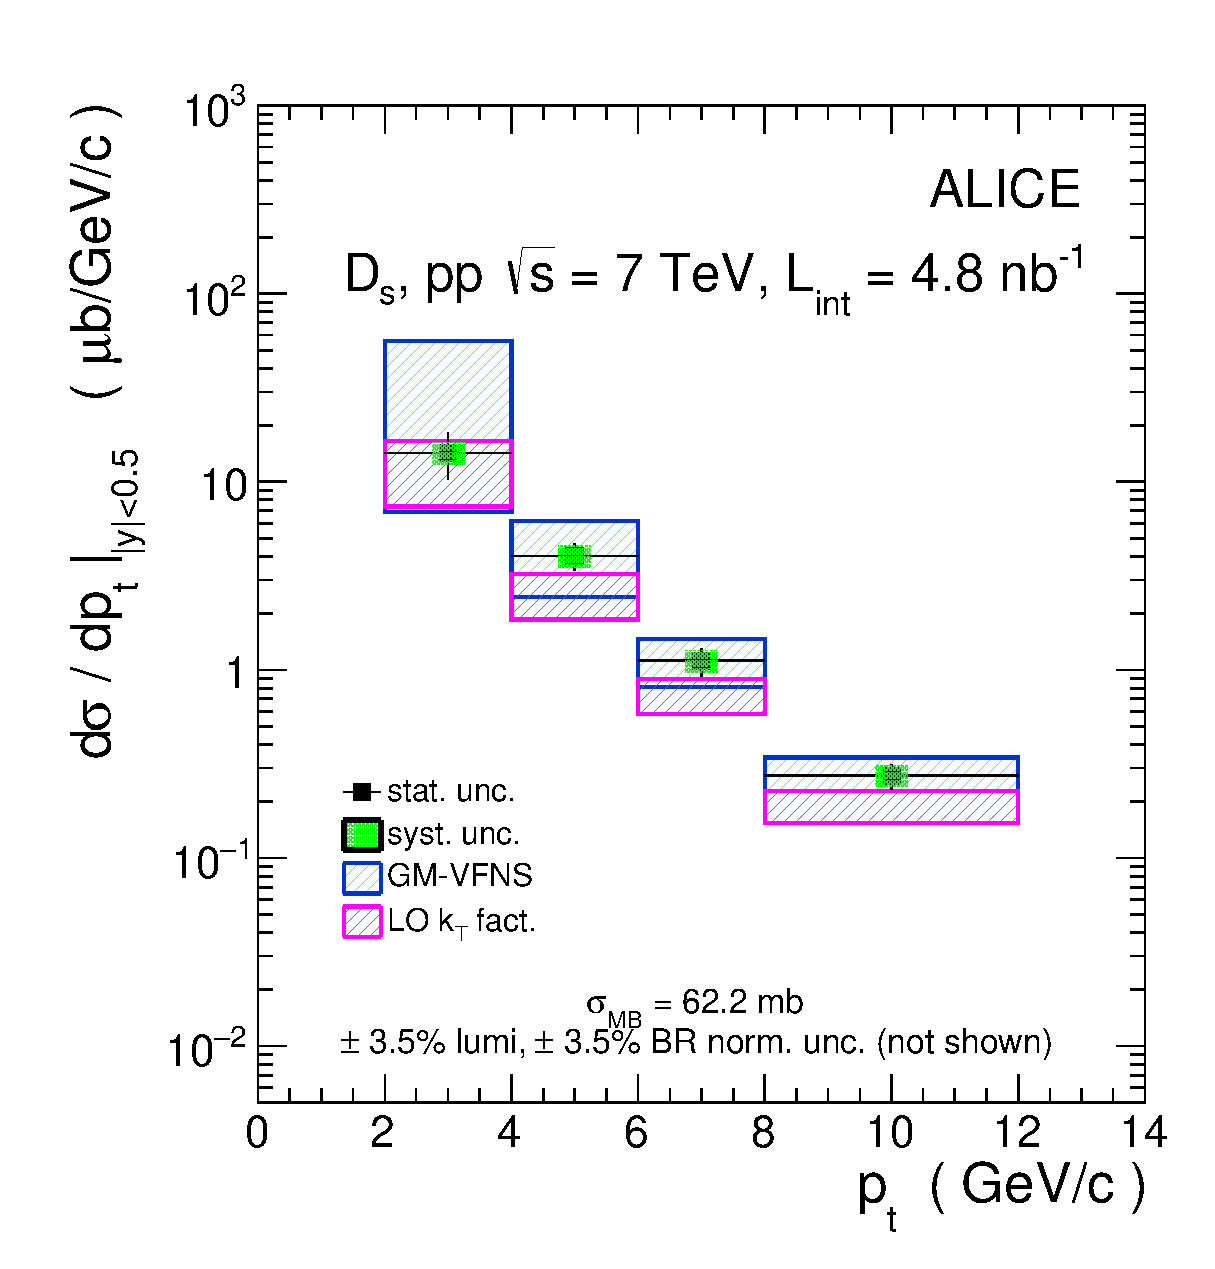
\includegraphics[width=.48\textwidth]{FigCap4/DsCrossModel.eps}
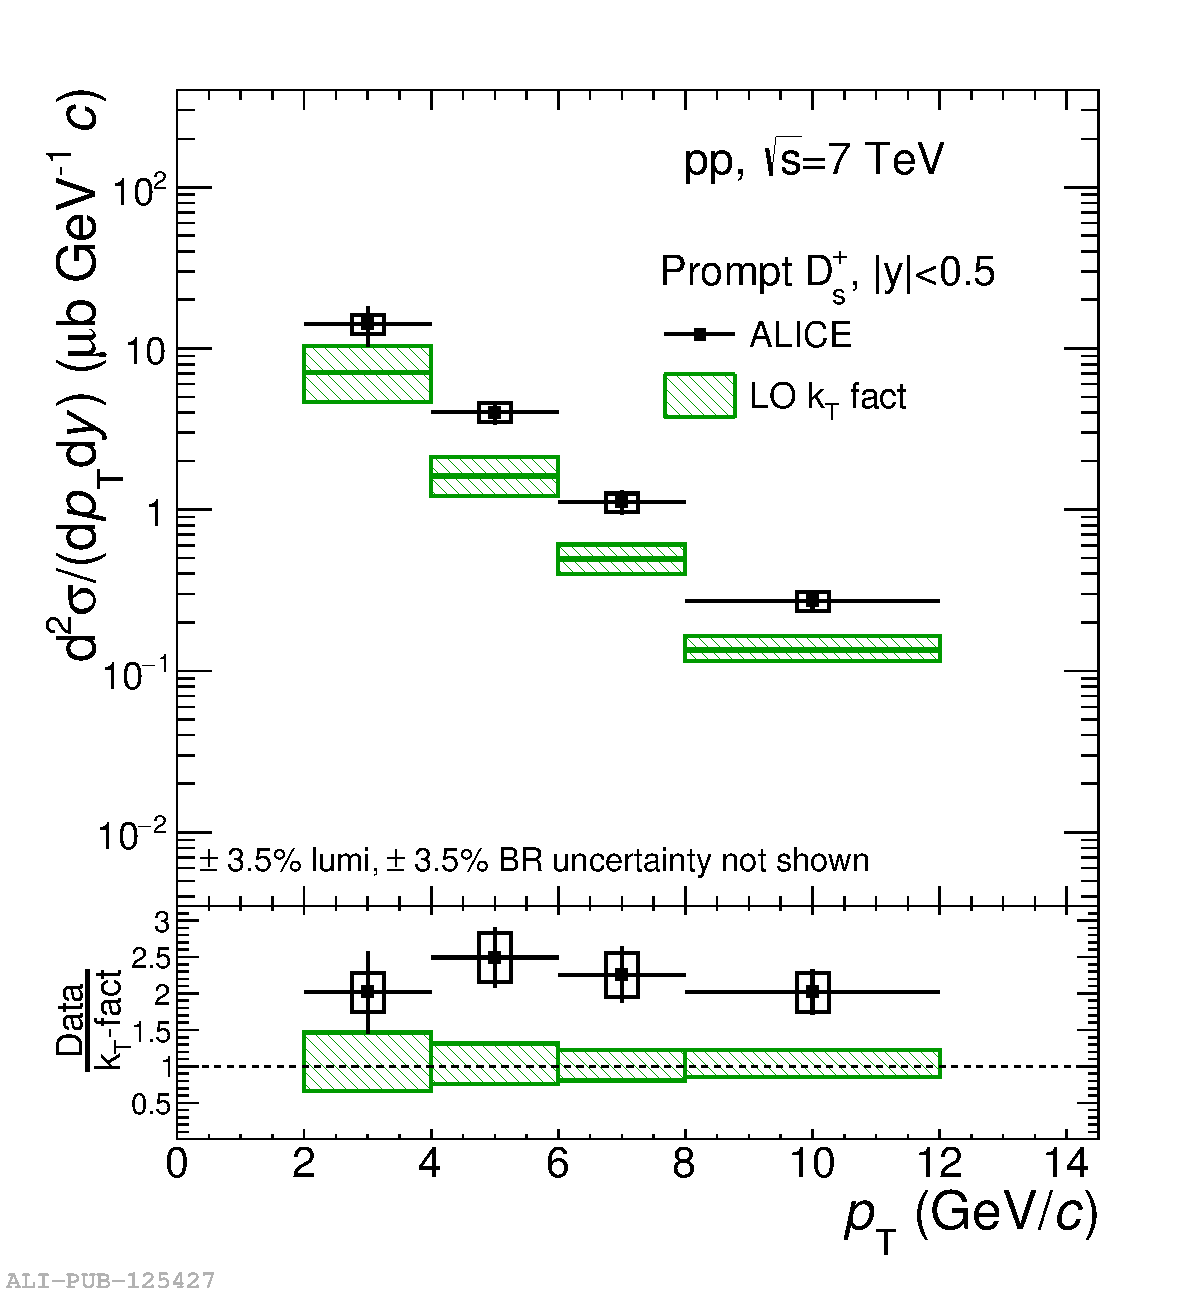
\includegraphics[width=.48\textwidth]{FigCap4/DsppCrossSecVsKtFactAndRatio.pdf}
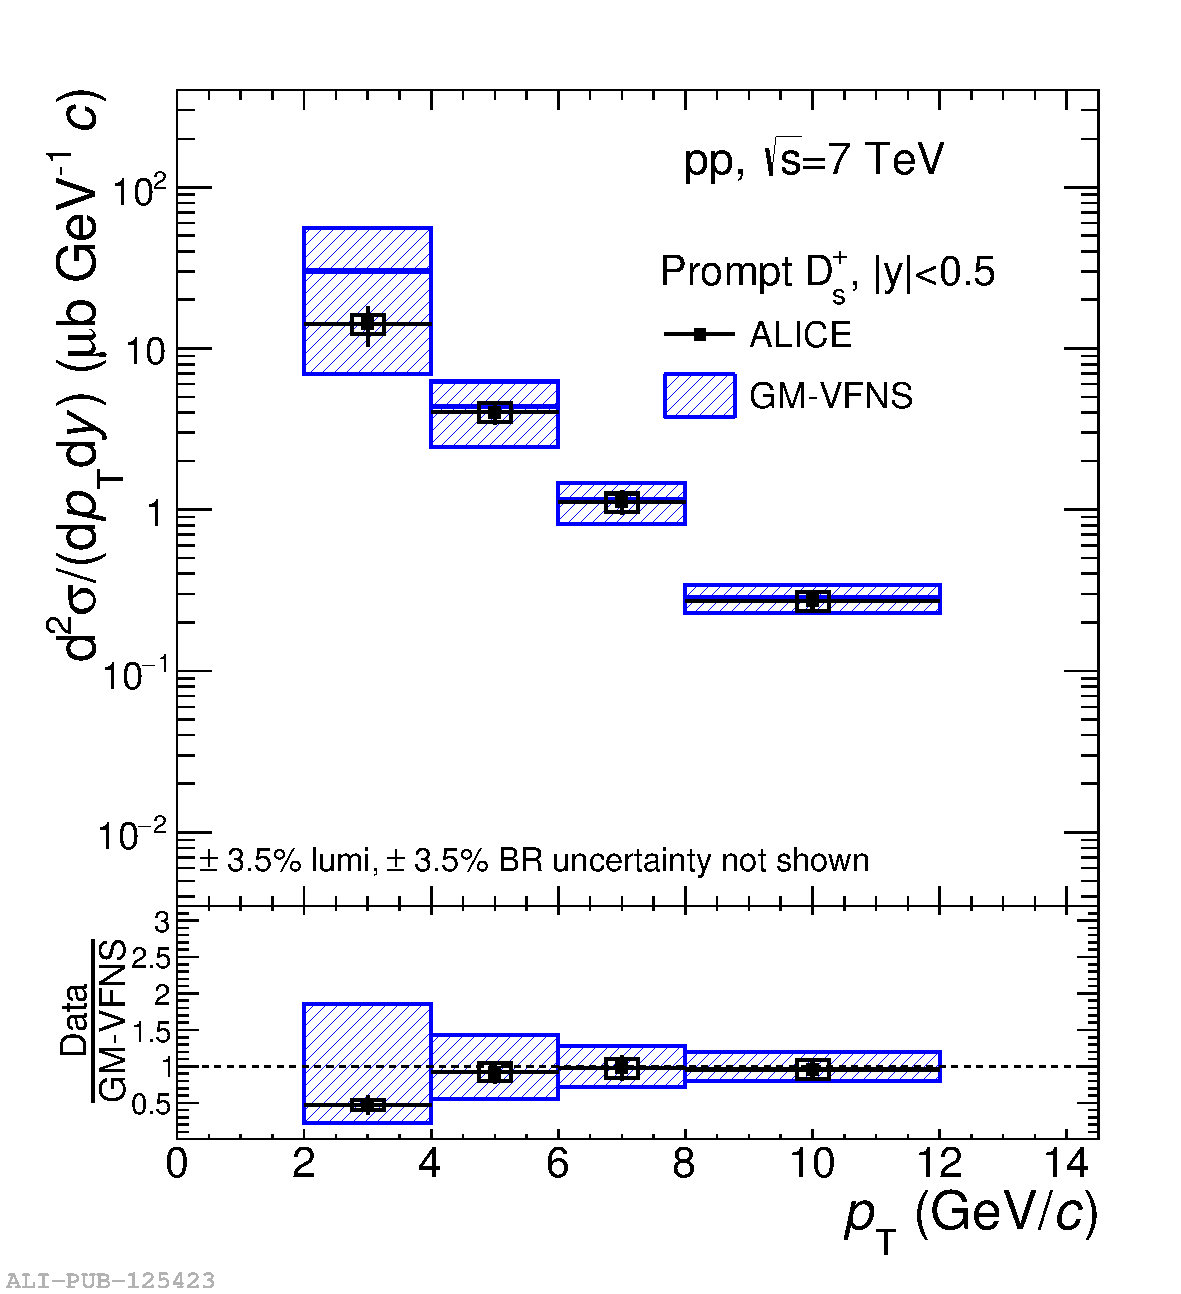
\includegraphics[width=.48\textwidth]{FigCap4/DsppCrossSecVsGMVFNSAndRatio.pdf}
\caption{Prompt $\Ds$-meson production cross section compared
to GM-VFNS calculations.}
\label{fig:CrossSecDsvsGMVFNS}
\end{center}
\end{figure}


In Fig.~\ref{fig:RatiosPass4}, the
 $\Dplus$/$\Dzero$, $\Ds$/$\Dzero$, $\Ds$/$\Dplus$ 
 meson production in pp pass4 are shown
as a function of $\pt$.
In Fig.~\ref{fig:RatiosPass2Pass4}, the same ratios are 
shown compared to published measurements in pass2, with an effective reduction of 
statistical and systematic uncertainties. 

\begin{figure}[!htb]
\begin{center}
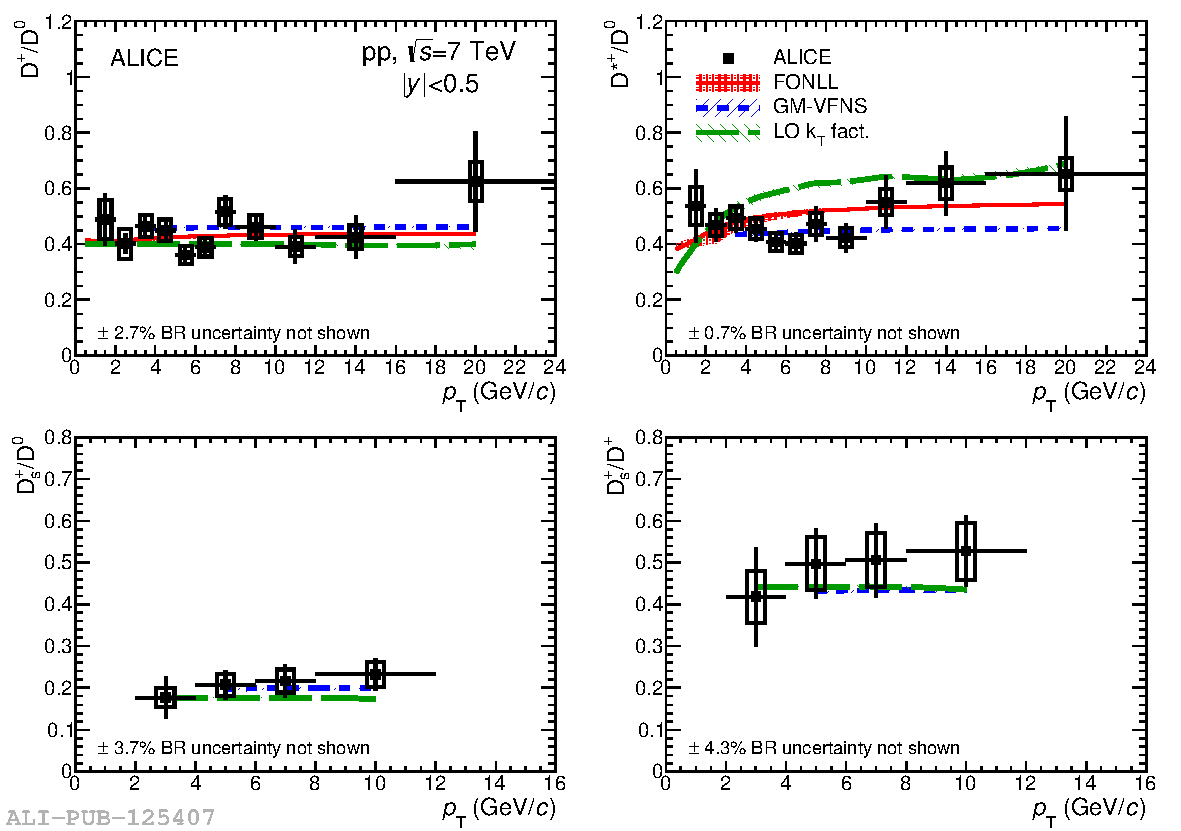
\includegraphics[width=1\textwidth]{FigCap4/DmesonRatiosVsModels.pdf}
\caption{D-meson production ratios in pp pass4 compared to the published results in pass2.}
\label{fig:RatiosPass2Pass4}
\end{center}
\end{figure}


